\documentclass{DeustoFDP}

\usepackage{hologo} % Paquete no necesario. Borrar en la memoria final al sustituir el texto
\usepackage{eurosym}
\usepackage{placeins}
\usepackage[toc, acronym, nomain]{glossaries}

\setlength{\headheight}{12.22504pt}

\hypersetup{
  pdfauthor={Unai Alonso \'Alvarez'},
  pdftitle={Dise\~no e implantaci\'on de un videojuego 2D con niveles creados proceduralmente'},
}

\bibliography{bibliografia}
\makeglossaries

\begin{document}

\newacronym{api}{API}{Application Programming Interface}
\newacronym{smfl}{SFML}{Simple and Fast Multimedia Library}
TCP
UDP
SDL
2D
ISO
JSON
FSF
LLVM
XML
TGUI

\frontmatter 
\pagestyle{plain}

% Las siguientes lineas (21--26) se pueden eliminar del documento final.
% Notese que en ese caso es necesario descomentar la linea 28 para que las
% paginas esten correctamente numeradas.
\begin{titlepage} 
  \newgeometry{left=0cm,right=0cm,bottom=0cm,top=0cm}
  
\includegraphics{fig/portada_rendered}
  \restoregeometry
\end{titlepage}
\cleardoublepage

%\setcounter{page}{3}

\chapter*{Resumen}

Hoy en día, la industria del videojuego o entretenimiento digital está en pleno auge, y es una opción laboral más que válida. Sin embargo, al ser un área con tanta gente aficionada, existen muchos proyectos y empresas dedicadas a ello, y su número está aumentando. Por este motivo, la competitividad es muy grande para los nuevos proyectos que surjan, y es difícil hacerse un hueco en la industria. A pesar de que existen varias ofertas educativas para formarse en el tema y así introducirse en el mercado laboral, los expertos coinciden en que la manera más eficaz de dar el salto es creando juegos. Este proyecto apunta a crear un producto que, además de servir como currículum, pudiera ser comercializable.

\vspace{2em}

{\Large\bfseries\sffamily Descriptores}
\vspace{3\medskipamount}

Videojuego, \acrshort{sfml}, generación procedural, Linux, Action \acrshort{rpg}

\cleardoublepage\tableofcontents
\cleardoublepage\listoffigures
\cleardoublepage\listoftables
\cleardoublepage\lstlistoflistings

\mainmatter
\pagestyle{phdthesis}

\chapter{Introducción}\label{cha:introduccion}

\section{Presentación del Documento}

El presente informe describe el proyecto de desarrollo Gestión de repositorios semánticos compatible con el estándar \acrshort{oaipmh}, un aplicativo que pretende extender a \acrshort{labman}, el \acrlong{dms} de los grupos de Internet y Telecomunicaciones de DeustoTech, detallando tanto los objetivos que se pretenden alcanzar con el proyecto, como las fases, actividades y recursos necesarios para llevarlo a cabo.

El contenido de este documento se estructura en torno a los siguientes productos:

\begin{itemize}
	\item \textbf{Definición de proyecto:}
		
	Establecimiento del objetivo fundamental del proyecto, especificando cuáles son los aspectos funcionales que lo comprenden y cuáles son los que quedan excluidos.
	
	\item \textbf{Producto final:}
		
	Especificación de la solución elegida que va a construir el proyecto en cuestión.
	
	\item \textbf{Descripción de la realización:}

	Realización y definición de las diferentes actividades cuyo desarrollo va a permitir la realización y consecución del objetivo del proyecto.

	\item \textbf{Organización:}
	
	Definición del equipo de trabajo que desarrollará el proyecto, así como su estructura organizativa, sistema de gestión y seguimiento del trabajo.

	\item \textbf{Condiciones de ejecución:}

	Definición del entorno de trabajo, de los criterios sobre los que se van a realizar las sucesivas recepciones, así como el tratamiento que se va a establecer para aquellos casos que puedan ser considerados como modificaciones o mejoras en el planteamiento inicial del proyecto.

	\item \textbf{Planificación:}
	Estimación de cargas y duración de las diferentes actividades del proyecto, así como su asignación a los diferentes miembros del equipo y su planificación en el tiempo.

	\item \textbf{Valoración económica:}
	Determinación del valor correspondiente a este proyecto, de los hitos de facturación y de la forma de pago.
\end{itemize}

\section{Introducción a LabMan}

Es este apartado se realiza una breve introducción a \acrfull{labman}, el \acrlong{dms} de MoreLab, el grupo de investigación formado por los equipos de Internet y Telecomunicaciones de DeustoTech y en el que se basa este proyecto.

\begin{figure}[!htp]
	\centering
	
\includegraphics[scale=0.15]{fig/morelab-logo}
	\caption{Logo de MORELab}
\end{figure}

Gestionar la información no siempre es una tarea trivial y más aún cuando hay que tratar con los datos que componen varias entidades como pueden ser los proyectos, investigadores, publicaciones, eventos, etc. dentro del ámbito de la investigación. La mayoría de los grupos de investigación utilizan sistemas de gestión de contenido tales como Joomla!\cite{joomla}, WordPress\cite{wordpress} o Drupal\cite{drupal} para exponer sus datos. Sin embargo, para extraer la información de estos \acrshortpl{cms} se requieren herramientas externas para llevar a cabo técnicas de análisis de datos. 
Para hacer uso de estas herramientas normalmente hace falta generar documentos adicionales, tales como \acrshort{csv}, hojas de cálculo, ficheros de texto, generado información redundante, que provoca dificultades a la hora de actualizar los datos y la calidad de los mismos. Esta situación empeora cuando además se disponen de distintas fuentes para la obtención de información, como pueden ser las paginas web personales de los investigadores en los que se muestran sus logros a lo largo de su carrera, la información financiera gestionada por su propio departamento, etc.

\begin{figure}[!htp]
	\centering
	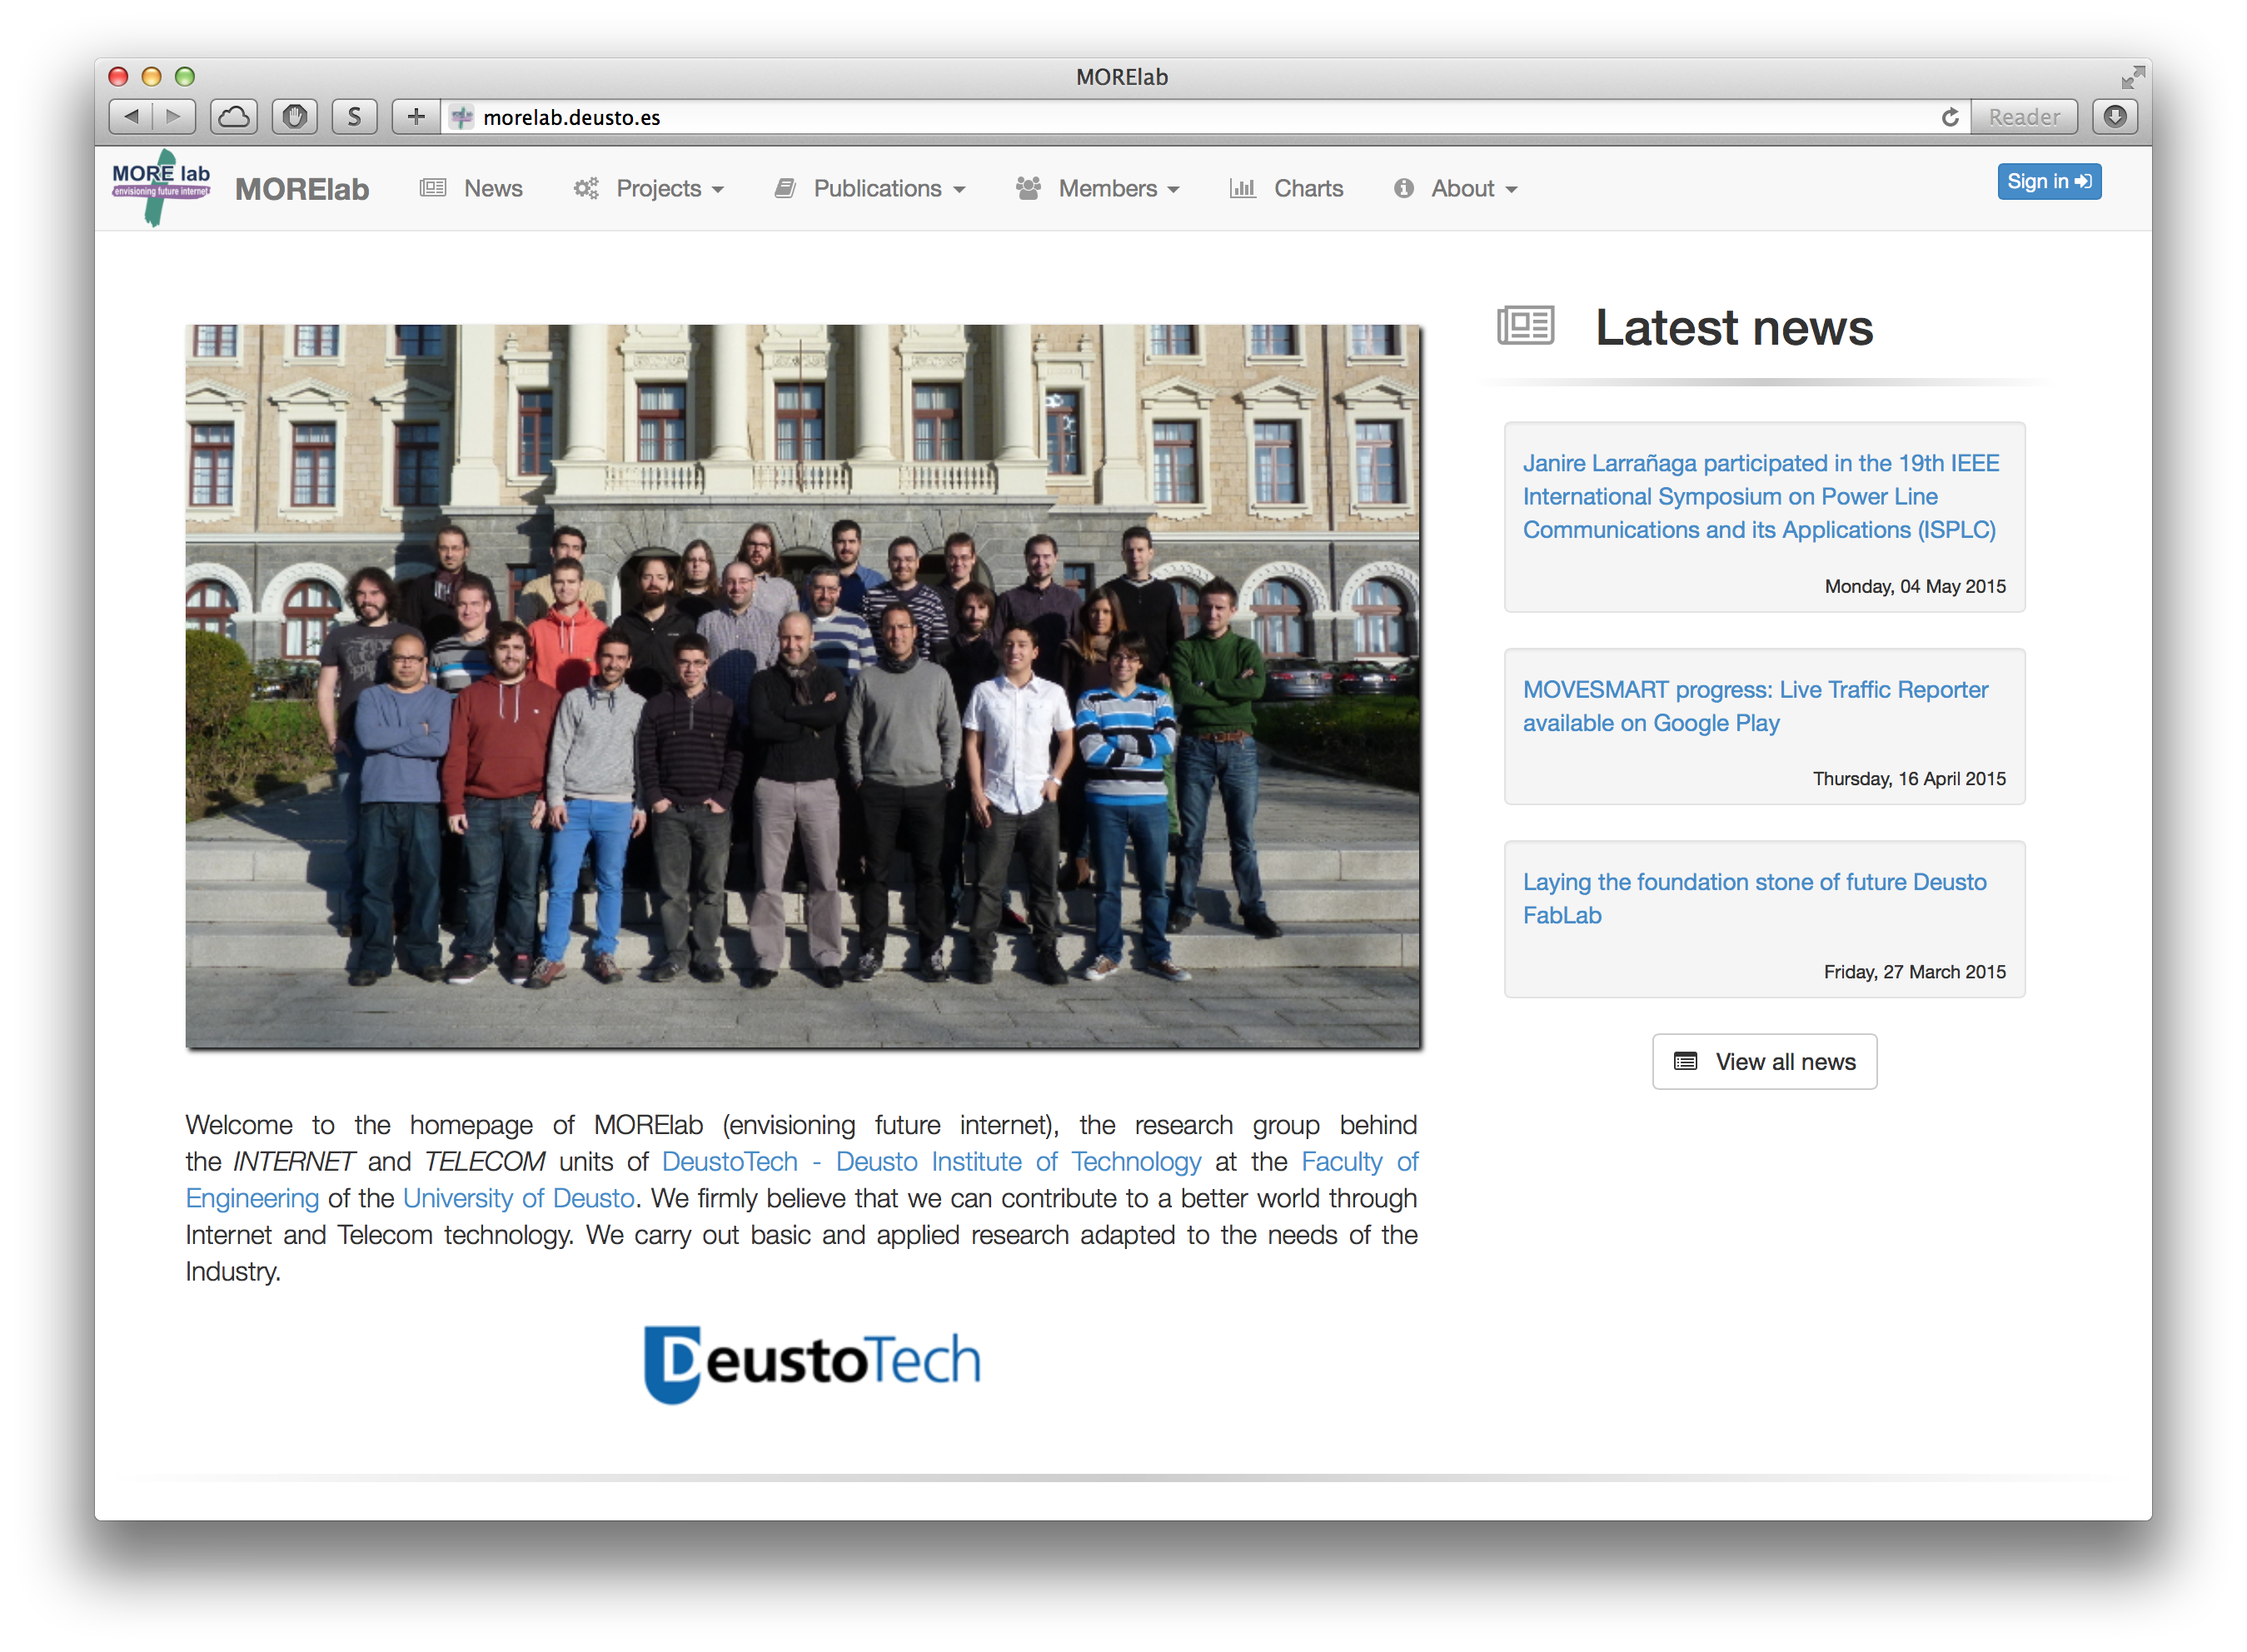
\includegraphics[scale=0.13]{fig/labman-homepage}
	\caption{Página de inicio de \acrshort{labman} con el equipo}
\end{figure}

Del esfuerzo para gestionar la información grupo de investigación de MoreLab nace \acrshort{labman}, una aplicación desarrollada en Python\cite{Python} por medio del framework para desarrollo web Django\cite{Django} y que sustituye a la antigua solución Joomla! para la publicación de los datos sobre las publicaciones en \acrshortpl{rdf}\cite{RDF}. Su principal objetivo es gestionar todo este tipo información, diferenciadose de otros \acrshortpl{cms} por apostar por la exposición de los datos como \acrlong{lod}\cite{linkeddata}, disponible por todos sin restricción de derechos de \textit{copyrights} o patentes.

Mediante el uso de los datos enlazados se es posible identificar cada entidad por medio de una \acrshort{uri}, permitiendo la creación de relaciones entre distintas instancias, lo que deriva en la posibilidad de descubrir patrones dentro de un set de datos.



\cite{pena_visual_2014}

\section{Motivación}

DeustoTech cree que es posible contribuir a un mundo mejor mediante el uso de las tecnologías de Internet y Telecomunicaciones.

Como resultado de este pensamiento nació \acrshort{labman}, un sistema de gestión de grupos de investigación. Esta aplicación web tiene como objetivo gestionar toda la información referente a los investigadores, proyectos y publicaciones de un grupo relacionada entre si. Permite generar diversas gráficas que permiten analizar de forma rápida la evolución y desempeño del grupo de investigación.

Este aplicativo es un claro ejemplo de una web de datos de nueva generación de portales web, dónde no solo se exportan documentos, sino que habilita la exportación datos y \acrshortpl{api}, que tienen como propósito facilitar la explotación de datos.

Aunque es capaz de exportar esta información semántica, todavía se ve la necesidad de que el sistema colabore con sistemas imperantes en la industria para el intercambio de información de recursos académicos y científicos.
Es por ello que se desea dar soporte a \acrshort{oai}, mediante la implementación de su protocolo \acrlong{oaipmh}, más comúnmente conocido por sus siglas \acrshort{oaipmh}, para poder comunicarse y dar servicio a soluciones del sector que apostaron por esta tecnología, favoreciendo por otra parte una mayor explotación de la información.

Así mismo se desea fomentar accesibilidad a dichos recursos, teniendo en especial consideración a aquellos usuarios que no disponen de conocimientos informáticos, por medio de un cliente web que sirva tanto de buscador como de filtrador.

Esta accesibilidad se garantizará mediante un estudio exhaustivo de los distintas formas en las que se pueden disponer los formularios y de cómo el usuario interactúa con ellos, teniendo como resultado una interfaz de usuario que asegura una experiencia intuitiva.

\chapter{Objetivos del proyecto}

\section{Definición del proyecto}

\subsection{Objetivos}

La gestión de repositorios semánticos compatibles con el estándar \acrshort{oaipmh} tiene como objetivo explotar la información almacenada en un repositorio de manera más eficiente, mediante consultas semánticas y facetadas avanzadas. Busca dar soporte a \acrshort{oaipmh} para disponer de todo el contenido según dicta su estándar.

Como caso práctico se propone añadir compatibilidad con \acrshort{oaipmh} al sistema de gestión de grupos de investigación LabMan, para que pueda proveer de datos a clientes que trabajen con esta tecnología.

Para dar sentido a esta funcionalidad, se pretende expandir labman con un cliente que se alimente con estos recursos para ofrecer servicios orientados a la búsqueda semántica y facetada.
\subsection{Alcance del proyecto}

Atendiendo a las premisas señaladas anteriormente, las funcionalidades que deberá soportar este proyecto serán:

\begin{itemize}
	\item Un servidor capaz de conectarse al repositorio de LabMan y extraer la información actualizada, en forma de metadatos, sobre las publicaciones y sus autores correspondientes de acuerdo con el estándar \acrlong{dc}\cite{DC}, respondiendo a las peticiones \acrshort{http} de acuerdo con el protocolo \acrshort{oaipmh}.
	
	\item Un cliente web capaz de realizar consultas semánticas y facetadas complejas y presentarlas intuitivamente a los usuarios, compuesto por formularios que se dispondrán de forma sencilla en primera instancia, para dar la posibilidad de realizar consultas rápidas y simples sin abrumar a los usuarios por la longitud del mismo. Pero, a su vez, han de permitir dar la posibilidad de expandir los campos con el fin de introducir datos más específicos para realizar consultas más elaboradas.

	\item La plataforma estará diseñada de una manera intuitiva, para que así, personas con pocos conocimientos de la informática también la puedan usar sin ningún tipo de problema. Además ha de ser responsiva, es decir, su diseño se adaptará a distintos tamaños de pantallas como pueden ser las de un ordenador de sobremesa, un portátil, una tableta o un móvil, donde poder plasmar toda la información de una manera legible para los humanos.
\end{itemize}

El proyecto se centrará solamente en el repositorio de Labman, a las tablas relacionadas a las publicaciones (Autores, Tesis, Libros, Tags, etc.), la incorporación de los demás repositorios de DeustoTech quedan aplazados para futuras revisiones del proyecto una vez concluido este.
\subsection{Producto final}

El producto final se compone de dos sistemas diferentes:

El primero es un servidor de documentos \acrshort{xml}\cite{XML} en el esquema \acrshort{dc}, capaz de responder a las peticiones \acrshort{html} según el protocolo \acrshort{oaipmh}. Será capaz de proveer información variada acerca de las publicaciones de los miembros que conforman Morelab en DeustoTech.

Los datos que proporcionará serán:

\begin{itemize}
	\item Información sobre los autores.
	\item Información sobre las tesis.
	\item Información sobre los libros publicados.
	\item Información sobre las revistas.
\end{itemize}

La segunda es una página web desarrollada con tecnologías como \acrshort{html}5, \acrshort{css}3 y \acrshort{js} que hoy en día está en auge y están adquiriendo más y más importancia.

La información será plasmada en la web de modo que cualquier usuario pueda consultarla y filtrarla de forma esquematizada y ordenada.

El objetivo de la aplicación web es poder explotar los datos suministrados por el servidor \acrshort{oaipmh}, mediante formularios dinámicos, permitiendo realizar tanto búsquedas semánticas avanzadas como facetadas de los recursos facilitados tanto por el servidor de acrshort{oaipmh}, como los de \acrshort{sql} y \acrshort{sparql}.

Añadir que el diseño de la interfaz será resultado de un estudio de los distintas formas de disponer los elementos dentro de un formulario, manteniendo la armonía con los estilos implantados en el sistema actual de LabMan.

Por último destacar, que el diseño de la página web será responsiva, es decir, su diseño se adaptará a distintos tamaños de pantallas como pueden ser las de un ordenador de sobremesa, un portátil, una tablet o un móvil. Además, el funcionamiento de la página deberá ser totalmente intuitiva para que gente con pocos conocimientos de la informática también la pueda usar sin ningún tipo de problema.

\section{Descripción de realización}

\subsection{Método de desarrollo}

El proyecto se desarrollará mediante un sistema de fases, en las que el orden es algo vital puesto que cada una de las fases dependerá de la previa. Por tanto, las fases de la solución planteada serán las siguientes:

\begin{enumerate}
	\item \textbf{Análisis de las herramientas a usar:}

	En esta fase se analizarán todas las posibles herramientas que se pueden usar para el desarrollo del proyecto y se elegirán las más adecuadas de acuerdo a las necesidades del proyecto y a los conocimientos del equipo de trabajo.
	\item \textbf{Integración y modelado de datos:}

	Es la fase en la que se identificará y seleccionarán las tablas del repositorio de las que se extraerá la información para su adaptación a Dublin Core.
	\item \textbf{Creación del servidor de OAI-PMH:}

	Diseño e implementación servidor.
	\item \textbf{Creación de la aplicación web:}

	Diseño e implementación del front-end de la aplicación web. 
	\item \textbf{Validación técnica y de usabilidad:}

	Es la fase donde se realizarán las pruebas finales del sistema completo.
	\item \textbf{Documentación y despliegue en producción:}

	Es donde se terminará de redactar la documentación necesaria y se desplegará el producto.
\end{enumerate}
\subsection{Productos intermedios}

Los productos intermedios que se generarán en cada una de las fases son:

\begin{itemize}
	\item \textbf{Integración y modelado de datos:}
	\begin{itemize}
		\item Especificación y diseño de la base de conocimiento del servidor OAI-PMH.
	\end{itemize}
	\item \textbf{Creación parte servidora del sistema:}
	\begin{itemize}
		\item Módulo de proveedor de la base de conocimiento.
		\item Módulo de adaptación y almacenamiento del conocimiento en Dublin Core.
		\item Módulo de servicio de XMLs.
	\end{itemize}
	\item \textbf{Creación de la aplicación web:}
	\begin{itemize}
		\item Aplicación web del sistema.
	\end{itemize}
	\item \textbf{Validación técnica y de usabilidad:}
	\begin{itemize}
		\item Informe de evaluación del sistema
	\end{itemize}
\end{itemize}

% TODO change EDT location %

\subsection{EDT}

\begin{figure}[!htp]
	\centering
	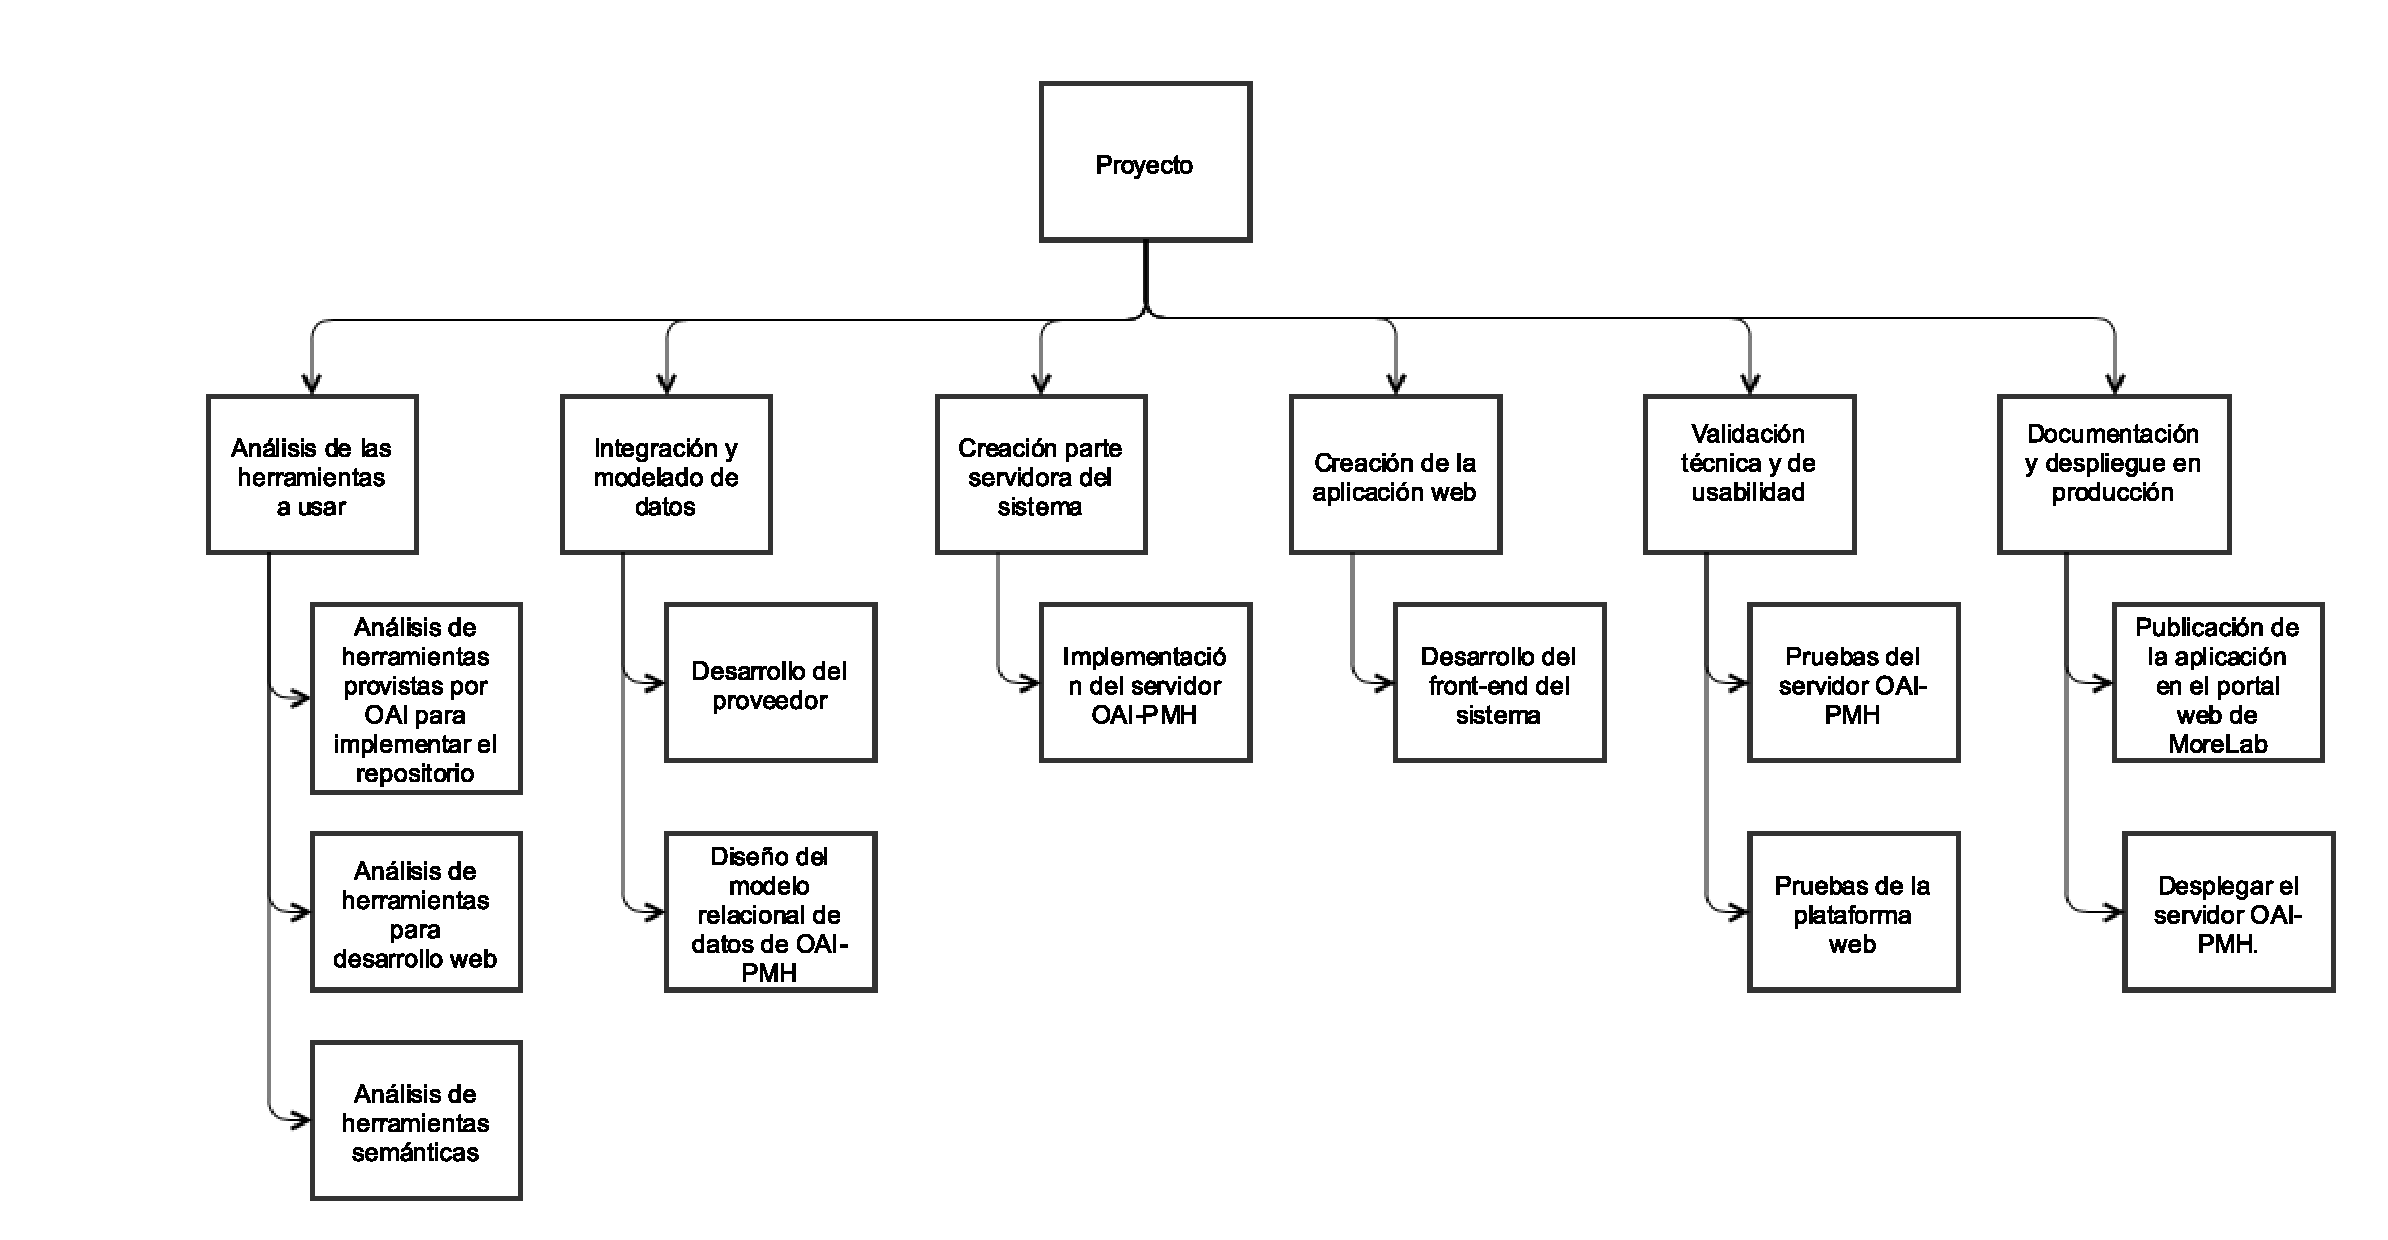
\includegraphics[angle=-90, scale=.5]{fig/edt}
	\caption{EDT}
\end{figure}

\subsection{Tareas principales}

La implantación del proyecto comprende las siguientes tareas o actividades: 

\subsubsection{Análisis de las herramientas a usar:}

\begin{itemize}
	\item \textbf{Análisis de herramientas provistas por OAI para implementar los requisitos mínimos para repositorio del protocolo OAI-PMH.}

	Investigar las distintas alternativas que hay para crear un servidor que beba de distintos tipos repositorios.
	\item \textbf{Análisis de herramientas para desarrollo web.}

	Investigar las distintas herramientas que hay para el desarrollo web y que sean adecuadas para el propósito del proyecto.
	\item \textbf{Análisis de herramientas semánticas.}

	Investigar las distintas alternativas para realizar búsquedas según los estándares de la web semántica. 
\end{itemize}

\subsubsection{Integración y modelado de datos:}

\begin{itemize}
	\item \textbf{Desarrollo del proveedor.}
	
	Desarrollo del sistema de extracción de datos de las tablas necesarias del repositorio PostgreSQL.

	\begin{enumerate}
		\item Formación: aprendizaje en el uso de las herramientas.
		\item Diseño: diseño del sistema de extracción de datos.
		\item Implementación: programación del sistema de extracción de datos.
		\item Pruebas: pruebas del sistema de extracción de datos.
	\end{enumerate}
	\item \textbf{Diseño del modelo relacional de datos de OAI-PMH.}
	\begin{enumerate}
		\item Diseño: diseño del modelo de la base de datos. 
		\item Implementación: inserción del modelo de datos en la base de datos.
		\item Pruebas: pruebas de la base de datos junto con el sistema de extracción de datos.
	\end{enumerate}
\end{itemize}

\subsubsection{Creación parte servidora del sistema:}

\begin{itemize}
	\item Implementación del servidor OAI-PMH.

	Puesta en marcha del servidor OAI-PMH que transforma datos almacenados mediante un modelo relacional a Dublin Core.

	\begin{enumerate}
		\item Implementación: configuración del servidor.
		\item Pruebas: pruebas del servidor.
	\end{enumerate}
\end{itemize}

\subsubsection{Creación de la aplicación web:}

\begin{itemize}
	\item \textbf{Desarrollo del front-end del sistema.}
	\begin{enumerate}
		\item Formación en la herramienta de desarrollo web.
		\item Diseño básico de la plataforma web.
		\item Diseño del módulo de búsquedas semánticas.
		\item Diseño del módulo de búsquedas facetadas.
	\end{enumerate}	
\end{itemize}

\subsubsection{Validación técnica y de usabilidad:}

\begin{itemize}
	\item \textbf{Pruebas del servidor OAI-PMH.}
	\item \textbf{Pruebas de la plataforma web.}
\end{itemize}

\subsubsection{Documentación y despliegue en producción:}

\begin{itemize}
	\item \textbf{Publicación de la aplicación en el portal web de MoreLab.}
	
	Instalar la aplicación web en el servidor de LabMan y publicarlo en el portal web.
	\item \textbf{Desplegar el servidor OAI-PMH.}

	Instalar el servidor OAI-PMH, recolectar y exportar la información del repositorio.
\end{itemize}

\section{Organización y equipo}

\subsection{Esquema organizativo}

La organización del proyecto se articula en torno al comité dirección y al equipo de trabajo que se va a encargar de desarrollar el producto, en función de la estructura de la figura 5.1.

\begin{figure}[!htp]
	\centering
	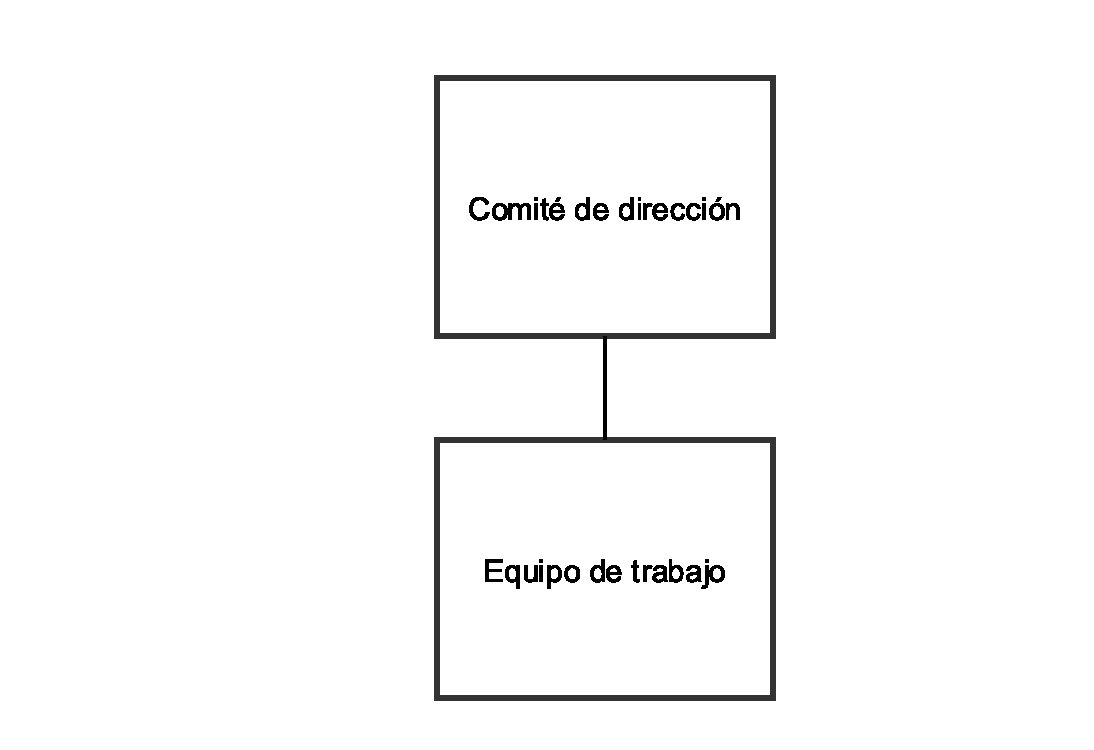
\includegraphics[scale=.75]{fig/organization}
	\caption{Esquema organizativo}
\end{figure}

\begin{itemize}
	\item Comité de dirección: su función principal es orientar por dónde debería ir el proyecto y tomar las decisiones finales a la hora de qué hacer o no.  Además, este comité deberá aprobar las diferentes fases del proyecto.
	\item Equipo de trabajo: el órgano encargado de diseñar y desarrollar el contenido del proyecto en función de las diferentes fases estipuladas.
\end{itemize}
\subsection{Plan de Recursos Humanos}\label{sec:planRecursosHumanos}

El equipo de trabajo estará formado por los siguientes perfiles directamente relacionados con las diferentes áreas de competencias que se abordan en el proyecto: 

\begin{itemize}
	\item Jefe de proyecto: su función es realizar las actividades de organización, coordinación y seguimiento del proyecto.
	\item Administrador de base de datos: su función es la de gestionar de una manera óptima la base de datos PostgreSQL y SPARQL y su función geoespacial. 
	\item Programador: su función es la desarrollar toda la lógica del programa como la implementación de la plataforma web. 
	\item Diseñador: su función es la diseñar interfaces intuitivas para el usuario y adaptables para distintos dispositivos (portátiles, tablets, móviles) 
	\item Experto en web semántica: su función es la de ayudar al equipo de trabajo a la hora de crear el sistema de búsquedas semánticas y facetadas. 
\end{itemize}

Debido a el bajo número de personas que compone el equipo de desarrollo se ha acordado trabajar mediante reuniones de seguimiento semanales pero también tras terminar cada tarea. En las reuniones semanales se reunirán todos los miembros del equipo, mientras que en las que corresponden a una tarea finalizada lo harán solo los que han participado en dicha tarea junto a el director de proyecto. Su finalidad será comentar los avances y/o problemas que hayan podido ocurrir, aunque también servirán para que el director de el visto bueno a la tarea y pasar a la siguiente. 

\section{Condiciones de ejecución}

\subsection{Entorno de trabajo}

El lugar de trabajo habitual serán las instalaciones de DeustoTech, aunque también se trabajará en casa para poder terminar a tiempo el proyecto.

El calendario y horario serán los correspondientes a los lugares de trabajo anteriormente mencionados durante una jornada laboral de aproximadamente 4 horas al día. Este horario podría verse modificado si se requiriera con el fin de cumplir los plazos establecidos.

En principio el director de proyecto será el responsable de todos los productos del desarrollo, y deberá dar el visto bueno a las herramientas que serán utilizadas para preservar las copias de seguridad y de definir cada cuanto tiempo deberán hacerse. En caso de que los desarrolladores no cumplan con estos requisitos y de producirse una perdida en el desarrollo serán estos los que asuman la responsabilidad, teniendo que optar por realizar horas extra o asumir de su sueldo la penalización que llegase a imponer el cliente en caso de no poder cumplirse con los plazos.

Los medios informáticos para la ejecución del proyecto deberán ser provistos por DeustoTech o serán los ordenadores personales de los integrantes del equipo. DeustoTech será responsable de todos los productos provistos para el desarrollo, salvo de aquellos medios pertenecientes a los propios desarrolladores. Los medios son los siguientes: 

\begin{itemize}
	\item Hardware
	\begin{itemize}
		\item Macbook Pro Retina 2012
		\item Servidor del repositorio Linux
		\item Monitor secundario
	\end{itemize}
	\item Software
	\begin{itemize}
		\item Licencia Sublime Text 2
		\item OS X
		\item Office 2011
		\item PostgreSQL
		\item SPARQL
	\end{itemize}
\end{itemize}
\subsection{Control de cambios}

Todas las peticiones que impliquen cambios en el diseño o en lo que ya está desarrollado, serán estudiadas y solo seguirán adelante si son modificaciones razonables y que son posibles de hacer dentro del plazo acordado. El procedimiento que habrá que seguir a la hora de  solicitar un cambio será:

\begin{enumerate}
	\item Comunicación de DeustoTech de las modificaciones solicitadas.
	\item Valoración por el equipo del proyecto de la repercusión técnica y cambios de plazos.
	\item Presentación de la decisión tomada por el equipo a DeustoTech.
	\item Notificación por parte de DeustoTech de la aprobación o no de la propuesta.	
	\item En caso afirmativo, modificación del plan de trabajo y del presupuesto.
\end{enumerate}
\subsection{Recepción de productos}

Para la recepción de productos el equipo del proyecto definirá una serie de pruebas que serán estrictamente ejecutadas. Una vez pasadas las pruebas, el jefe de proyecto deberá revisar y aceptar el producto para poder presentarlo oficialmente a DeustoTech.  En caso de que exista algún problema tras la revisión,  la dirección de DeustoTech-Internet deberá comunicarlo en un plazo máximo de 5 días para poder llevar a cabo las modificaciones y así poder seguir con la siguiente fase del proyecto. En caso de no obtener respuesta en el intervalo de tiempo especificado anteriormente, se considerará aprobado.

DeustoTech-Internet es el equipo de investigación centrado en el desarrollo web de la Universidad de Deusto. Este proyecto se ha delegado a varios de sus colaboradores de investigación. Dado a la estrecha relación que existen entre ambos no se han definido todos los requisitos desde el punto de partida, lo cual puede causar que retrasos en la fecha de entrega del producto. Sin embargo, al un proyecto interno no se le ha dado mayor importancia.

\section{Planificación}

\subsection{Diagrama de precedencias}

\begin{figure}[!htbp]
	\centering
	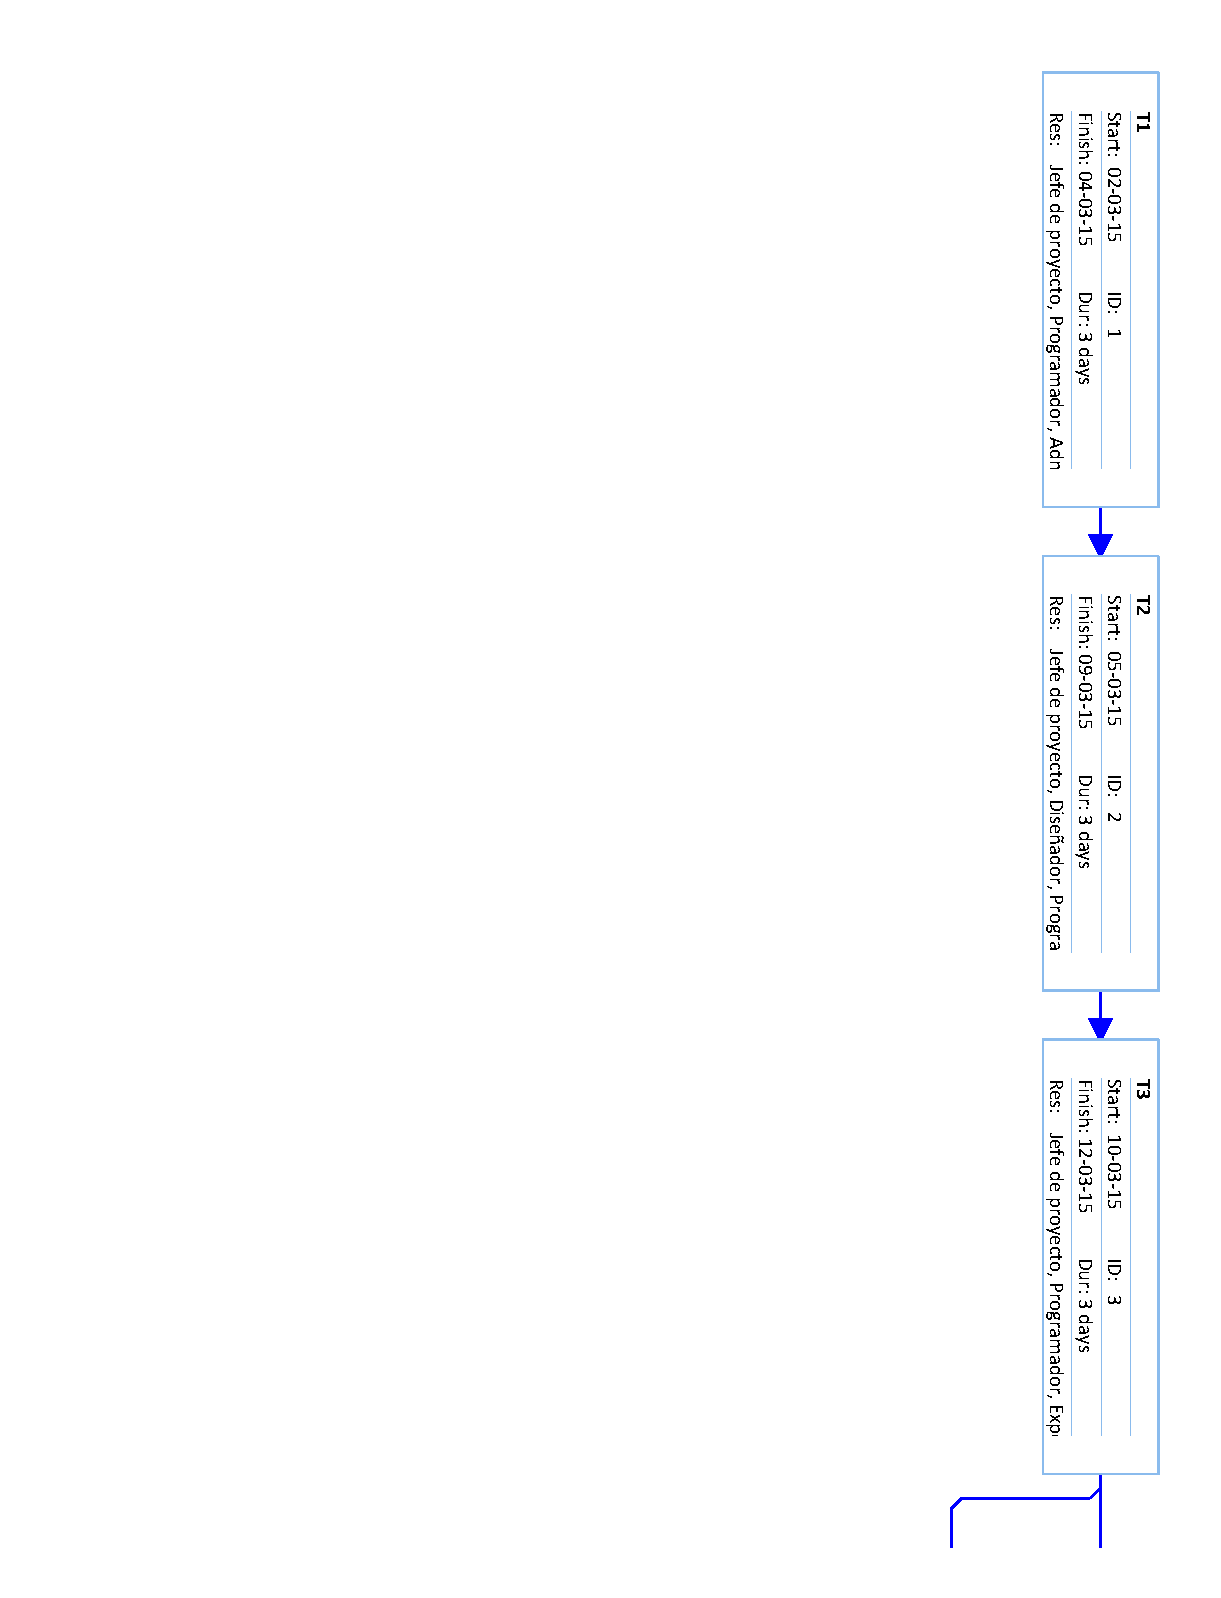
\includegraphics[page=1, scale=.65]{fig/network_diagram}
	\caption{Diagrama de precedencias 1}
\end{figure}

\begin{figure}[!htbp]
	\centering
	\includegraphics[page=2, scale=.65]{fig/network_diagram}
	\caption{Diagrama de precedencias 2}
\end{figure}

\begin{figure}[!htbp]
	\centering
	\includegraphics[page=3, scale=.65]{fig/network_diagram}
	\caption{Diagrama de precedencias 3}
\end{figure}

\begin{figure}[!htbp]
	\centering
	\includegraphics[page=4, scale=.65]{fig/network_diagram}
	\caption{Leyenda del diagrama de precedencias}
\end{figure}
\subsection{Plan de Trabajo}

TODO
\subsection{Diagrama de Gantt}

\begin{figure}[!htp]
	\centering
	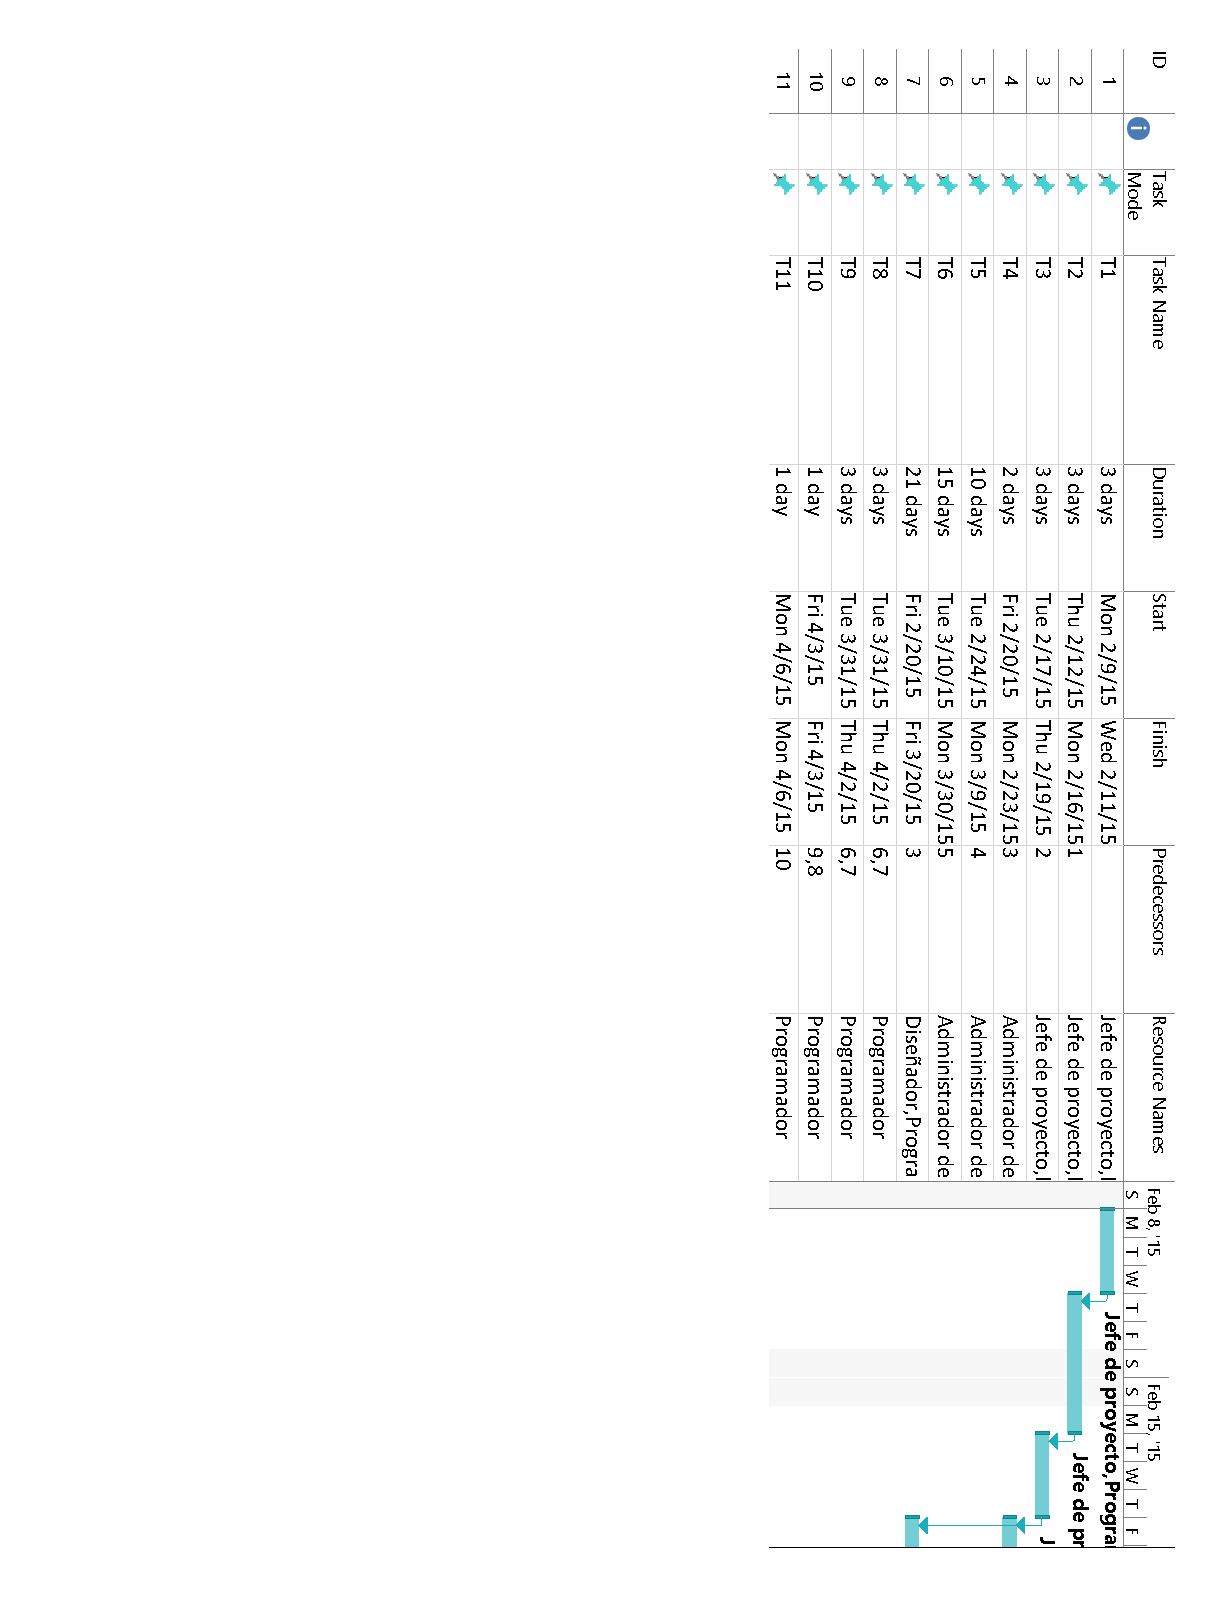
\includegraphics[page=1, scale=.7]{fig/gantt_diagram}
	\caption{Diagrama de Gantt 1}
\end{figure}

\begin{figure}[!htp]
	\centering
	\includegraphics[page=2, scale=.7]{fig/gantt_diagram}
	\caption{Diagrama de Gantt 2}
\end{figure}

\begin{figure}[!htp]
	\centering
	\includegraphics[page=3, scale=.7]{fig/gantt_diagram}
	\caption{Diagrama de Gantt 3}
\end{figure}

\begin{figure}[!htp]
	\centering
	\includegraphics[page=4, scale=.7]{fig/gantt_diagram}
	\caption{Leyenda del diagrama de Gantt}
\end{figure}
\subsection{Estimación de cargas de trabajo por perfil}

\begin{table}[htp]
	\centering
	\caption{Cargas de trabajo por perfil}\label{tab:workload}
	\begin{tabular}{cc}
		\toprule
    	\textbf{Perfil de trabajo} & \emph{Carga de trabajo(h)}\\
    	\midrule
		Jefe de proyecto & 6,05\\
		Administrador de base datos & 64,05\\
		Diseñador gráfico & 26,22\\
		Experto en web semántica & 26,\\
		Programador & 185,48\\
    	\bottomrule
    \end{tabular}
\end{table}

\section{Presupuesto}

\subsection{Recursos Humanos}

\begin{table}[htp]
	\centering
	\caption{Presupuesto: Recursos Humanos}\label{tab:budget-human}
	\begin{tabular}{cccc}
		\toprule
    	\textbf{Rol} & \emph{Precio/hora(\euro/h)} & \emph{Carga de trabajo(h)} & \emph{Importe total(\euro)}\\
    	\midrule
    	Jefe de proyecto				&	40			&	6,05 					& 	242,00\\
		Administrador de base de datos	&	25			&	64,05					&	1.601,25\\
		Programador						&	25			&	185,48					&	4.637,00\\
		Diseñador						&	15			&	26,22					&	393,30\\
		Experto en web semántica		&	30			&	26,22					&	786,60\\
    	\bottomrule
    \end{tabular}
\end{table}
\subsection{Recursos Software}

\begin{table}[htp]
	\centering
	\caption{Presupuesto: Software}\label{tab:budget-software}
	\begin{tabular}{cccc}
		\toprule
    	\textbf{Nombre} & \emph{Precio(\euro)} & \emph{Unidades} & \emph{Importe total(\euro)}\\
    	\midrule
    	Licencia Sublime Text 2		& 	70				&	1 			& 	70\\
    	Office 2011 				&	99				&	1			&	99\\
    	\bottomrule
    \end{tabular}
\end{table}
\subsection{Recursos Hardware}

\begin{table}[htp]
	\centering
	\caption{Presupuesto: Hardware}\label{tab:budget-hardware}
	\begin{tabular}{cccc}
		\toprule
    	\textbf{Nombre} & \emph{Precio(\euro)} & \emph{Unidades} & \emph{Importe total(\euro)}\\
    	\midrule
    	\acrshort{rmbp}2012			& 	3.334			&	1 			&	3.334					\\
    	Monitor secundario	&	300				&	1			&	300						\\
    	\bottomrule
    \end{tabular}
\end{table}
\subsection{Total}

\begin{table}[htp]
	\centering
	\caption{Presupuesto: Total}\label{tab:total-budget}
	\begin{tabular}{cc}
		\toprule
    	\textbf{Tipo} 		& 	\emph{Total}\\
    	\midrule
    	Recursos Humanos	& 			7.660,15\\
		Recursos Software	&			169,00\\
		Recursos Hardware	&			3.634,00\\
		\textbf{Total}		&	\textbf{11.463,15}\\
    	\bottomrule
    \end{tabular}
\end{table}
\chapter{Especificación de Requisitos}

\section{Visión general}

	En este capítulo se especifican los requisitos que deben ser cumplidos por el proyecto a desarrollar. Para un mejor entendimiento de los mismos, se han dividos en dos bloques:

	\begin{itemize}
			\item \textbf{Requisitos funcionales:}
				
			Funcionamiento que el juego debe proveer.
			
			\item \textbf{Requisitos no funcionales:}
				
			Requisitos relacionados con la usabilidad, el entorno y el rendimiento.
	\end{itemize}

\section{Requisitos funcionales}

	Requisitos funcionales que describen el funcionamiento del producto. A continuación se muestran los requisitos del juego:

	\begin{itemize}
			\item \textbf{RF0}
				
			El nivel que constará la demo debe ser generado proceduralmente en cada sesión y debe poblarse de enemigos.
			
			\item \textbf{RF1}
				
			El juego debe ser capaz de detectar cuando distintas entidades colisionan entre ellas o con el escenario y actuar en consecuencia.

			\item \textbf{RF2}
				
			La cámara del juego debe seguir al jugador en los ejes X e Y.

			\item \textbf{RF3}
				
			El juego debe detectar las entradas del jugador, comprobar el estado actual del mismo y actuar en consecuencia.

			\item \textbf{RF4}
				
			El juego debe detectar cuando se han cumplido las condiciones para fin de partida y terminarla.

			\item \textbf{RF5}
				
			Cada enemigo debe tener una inteligencia artificial distinta.

			\item \textbf{RF6}
				
			El jugador debe tener a su disposición tres tipos de ataque.

			\item \textbf{RF7}
				
			El juego debe contar con una pantalla para mostrar los controles.
	\end{itemize}

\section{Requisitos no-funcionales}
	
	Los requisitos no funcionales describen características requeridas del sistema, el proceso de desarrollo o cualquier otro aspecto que tenga alguna restricción.

	\subsection{Usabilidad}

		Estos requisitos permiten que el juego cumpla las espectativas del usuario final.

		\begin{itemize}
				\item \textbf{RU0}
					
				Durante las partidas el juego debe mostrar en todo momento los datos relevantes al usuario mediante una interfaz gráfica.

				\item \textbf{RU1}
					
				La interfaz gráfica debe estar diseñada de forma que no sea molesta para el jugador.

				\item \textbf{RU2}
					
				El juego debe controlarse únicamente con el teclado.
		\end{itemize}

	\subsection{Entorno}

		Estos requisitos definen el entorno de uso del juego.

		\begin{itemize}
				\item \textbf{RE0}
					
				El código del juego debe ser multiplataforma, de forma que pueda compilarse en Windows, Linux y OSX.

				\item \textbf{RE1}
					
				La versión final debe incluir las librerías necesarias para el correcto funcionamiento del juego.
		\end{itemize}

	\subsection{Rendimiento}

		Requisitos relacionados con el tiempo de realización de las tareas de la aplicación, márgenes de error...

		\begin{itemize}
				\item \textbf{RR0}
					
				El juego debe funcionar a un mínimo de 30 FPS en cualquier plataforma.

				\item \textbf{RR1}
					
				Durante las partidas, no debe haber errores que provoquen un final inesperado de la aplicación.
		\end{itemize}

\section{Criterios de validación}

	Los requisitos previamente mencionados están sujetos a procesos de validación antes de la entrega final del proyecto. Para comprobar el cumplimiento de los requisitos, el producto final es contrastado con los requisitos iniciales, estudiando los cambios que pudieran surgir. El método de desarrollo está guiado por pruebas, de forma que el cumplimiento exitoso de dichas pruebas validará los distintos requisitos del sistema objetivamente, mientras que si las pruebas no se ejecutan exitosamente indicarán la existencia de requisitos incompletos.

	El grado de incumplimiento del proyecto estará directamente relacionado con el porcentaje de requisitos cumplidos, evaluando el grado de completitud objetivamente.

	De la misma forma, cualquier implementación que mejore la estabilidad o funcionalidad del sistema que no esté reflejado en los requisitos iniciales se considerará una parte extra de la evaluación del proyecto por el director del mismo.
\chapter{Especificación del diseño}

\section{Visión general}

	En este capítulo se describe el trabajo de diseño realizado para el proyecto, así como el entorno y las herramientas que han sido utilizadas para llevarlo a cabo.

\section{Arquitectura}

	La arquitectura básica del juego es la que se muestra en la siguiente imagen. El usuario genera entradas al juego mediante el teclado, después estas entradas son procesadas por la lógica del juego y se realizan las acciones pertinentes en función del estado del juego. Una vez actualizado el estado del juego ha sido actualizado, los módulos de audio y vídeo generan las salidas correspondientes y las muestran mediante la pantalla y el dispositivo reproductor de audio actual.

	\begin{figure}[!htp]
		 \centering
		 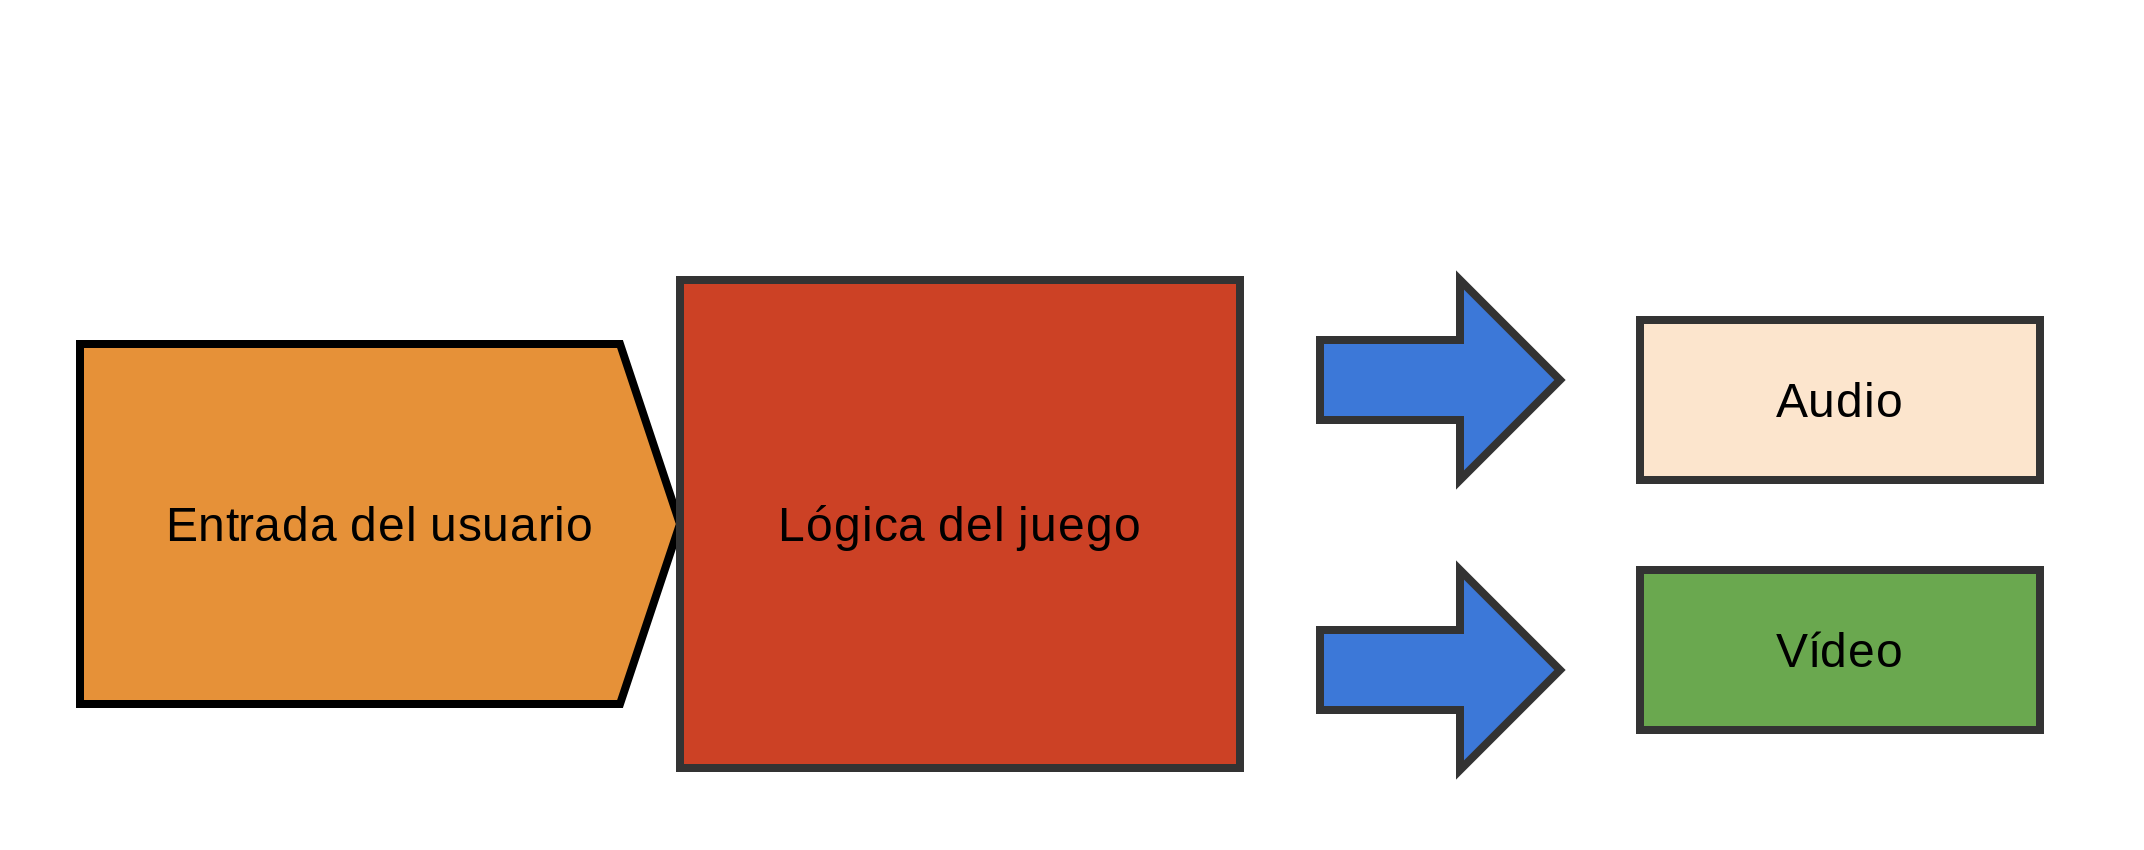
\includegraphics[scale=.15]{fig/architecture}
		 \caption{Diagrama de arquitectura}
		 \label{fig:arch}
	\end{figure}

	\FloatBarrier
	\clearpage

\section{Diagrama de clases}

	\begin{figure}[!htp]
		 \centering
		 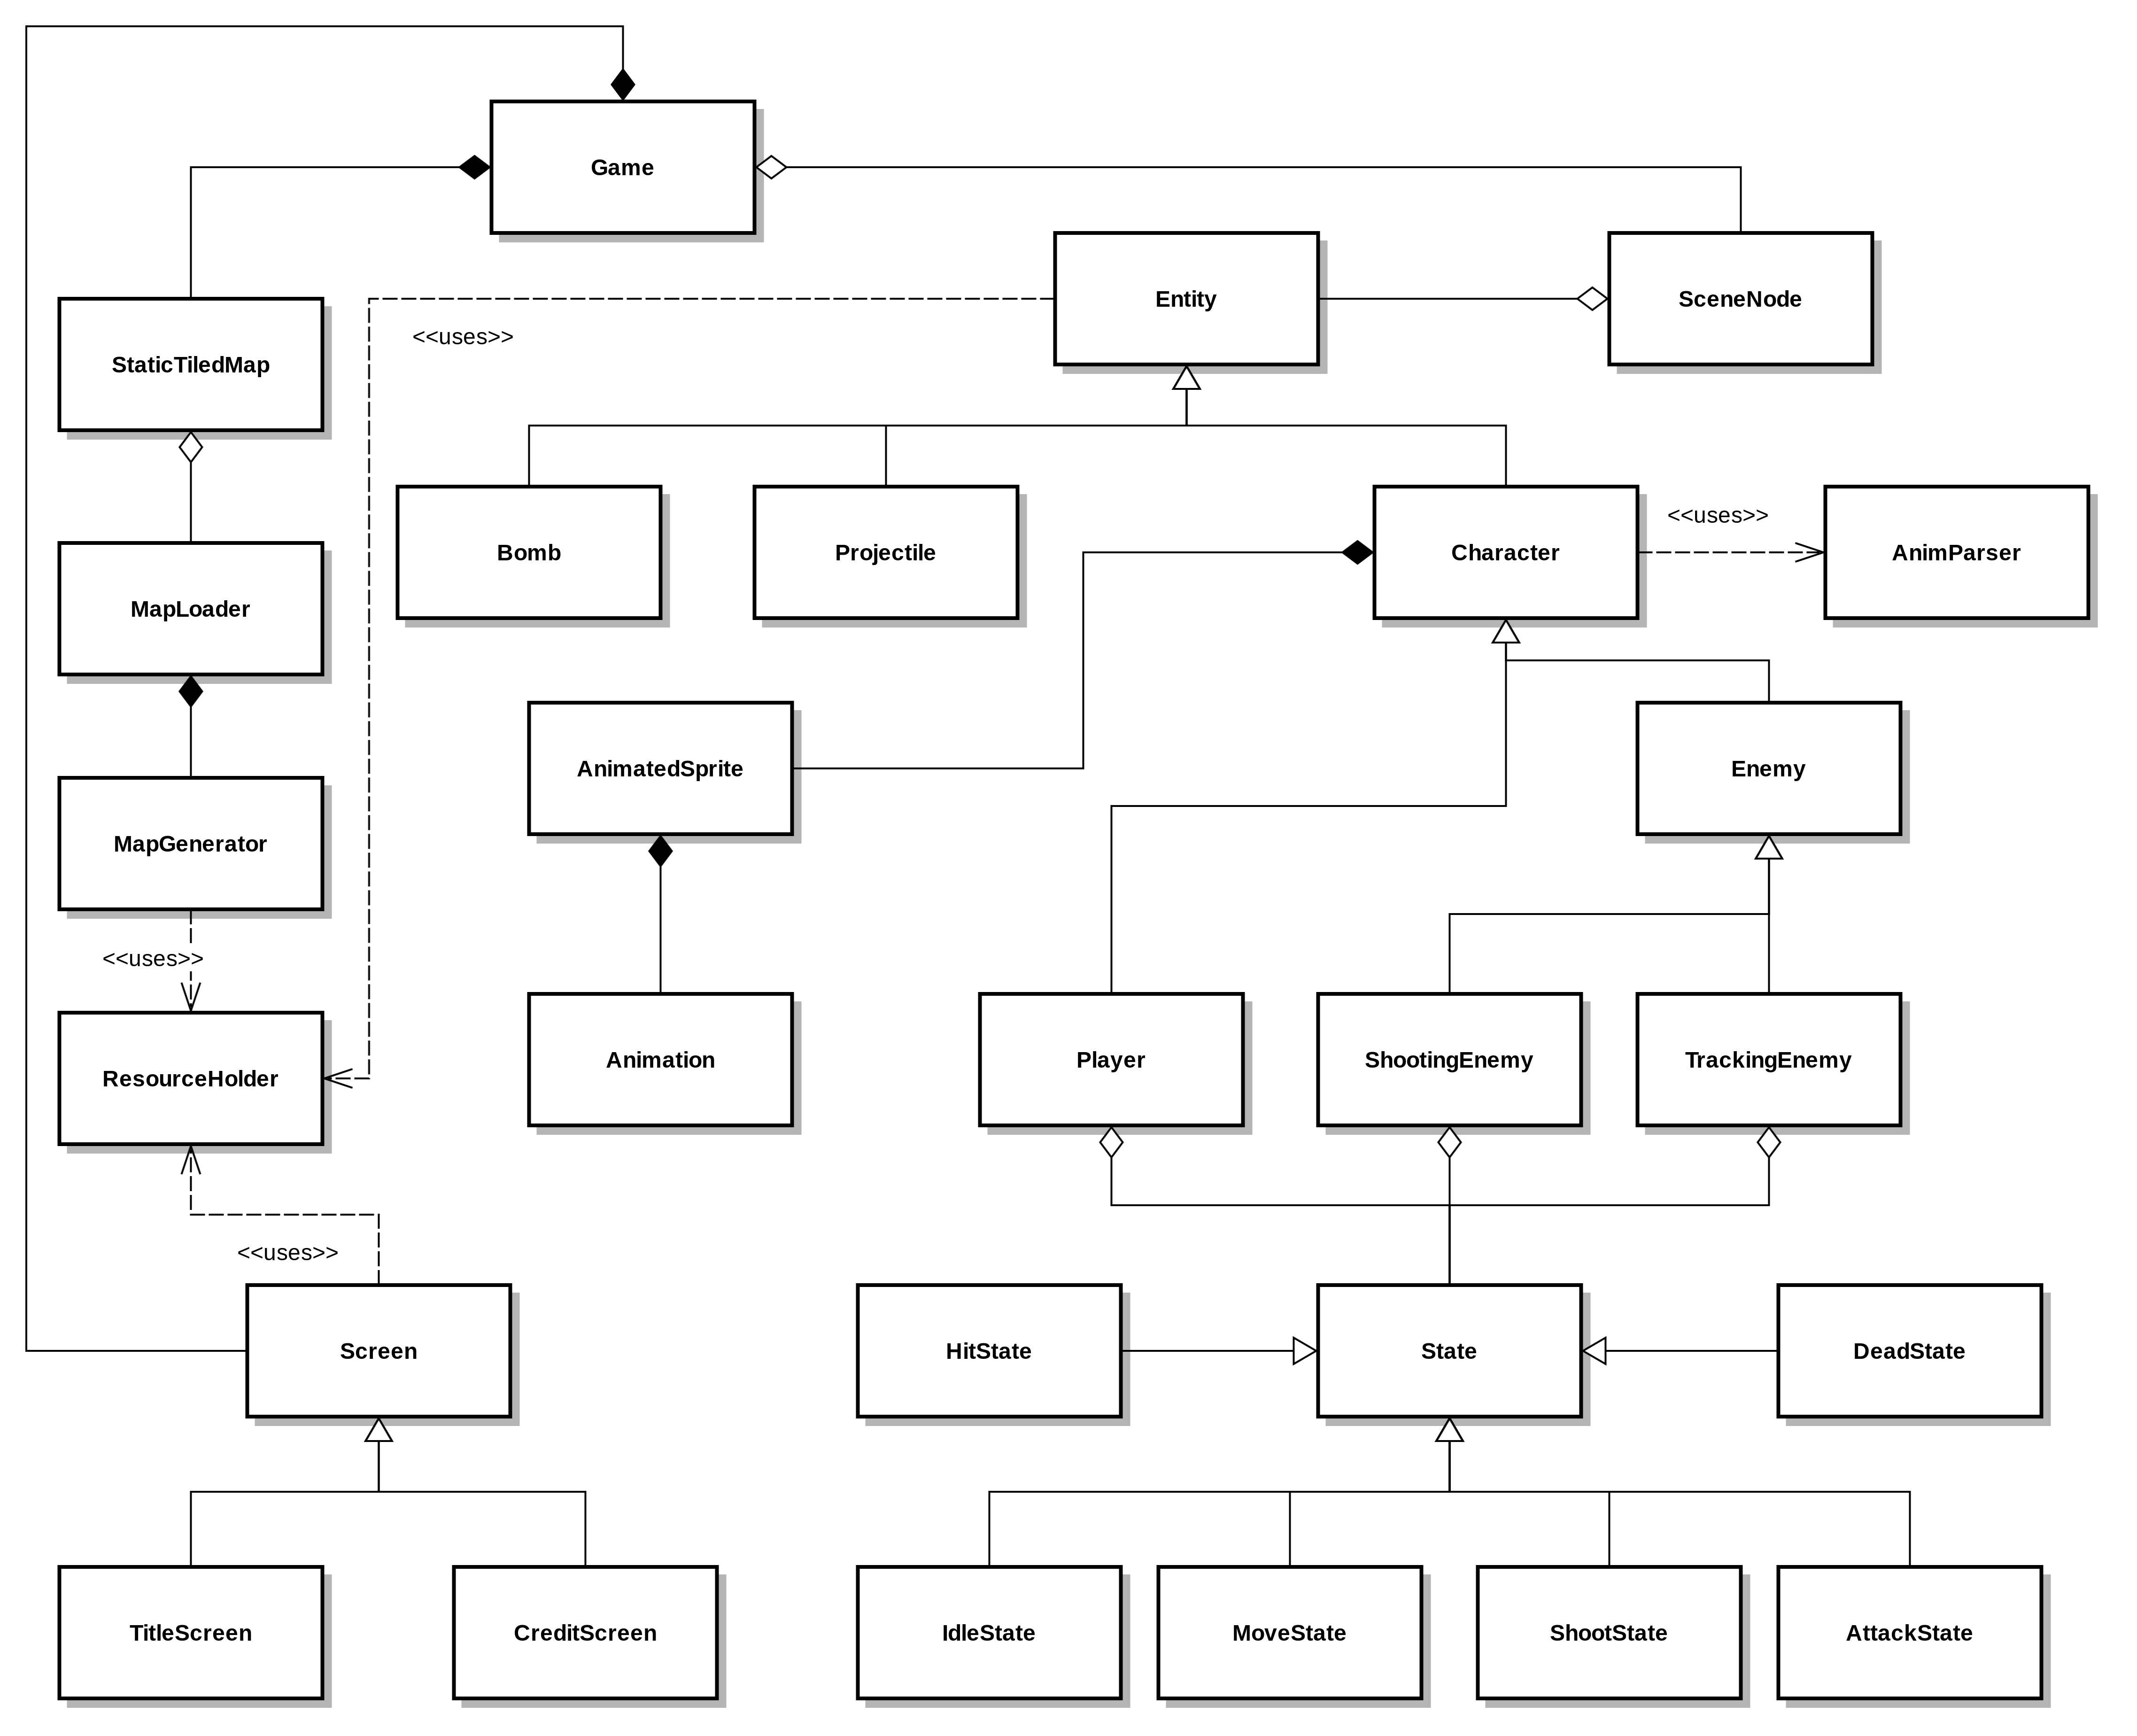
\includegraphics[scale=.08]{fig/class}
		 \caption{Diagrama de clases}
		 \label{fig:class}
	\end{figure}

	\FloatBarrier
	\clearpage

\section{Diagramas de actividad}

	A continuación se muestra el diagrama de actividad del programa desde que se ejecuta hasta que finaliza.

	\begin{figure}[!htp]
		 \centering
		 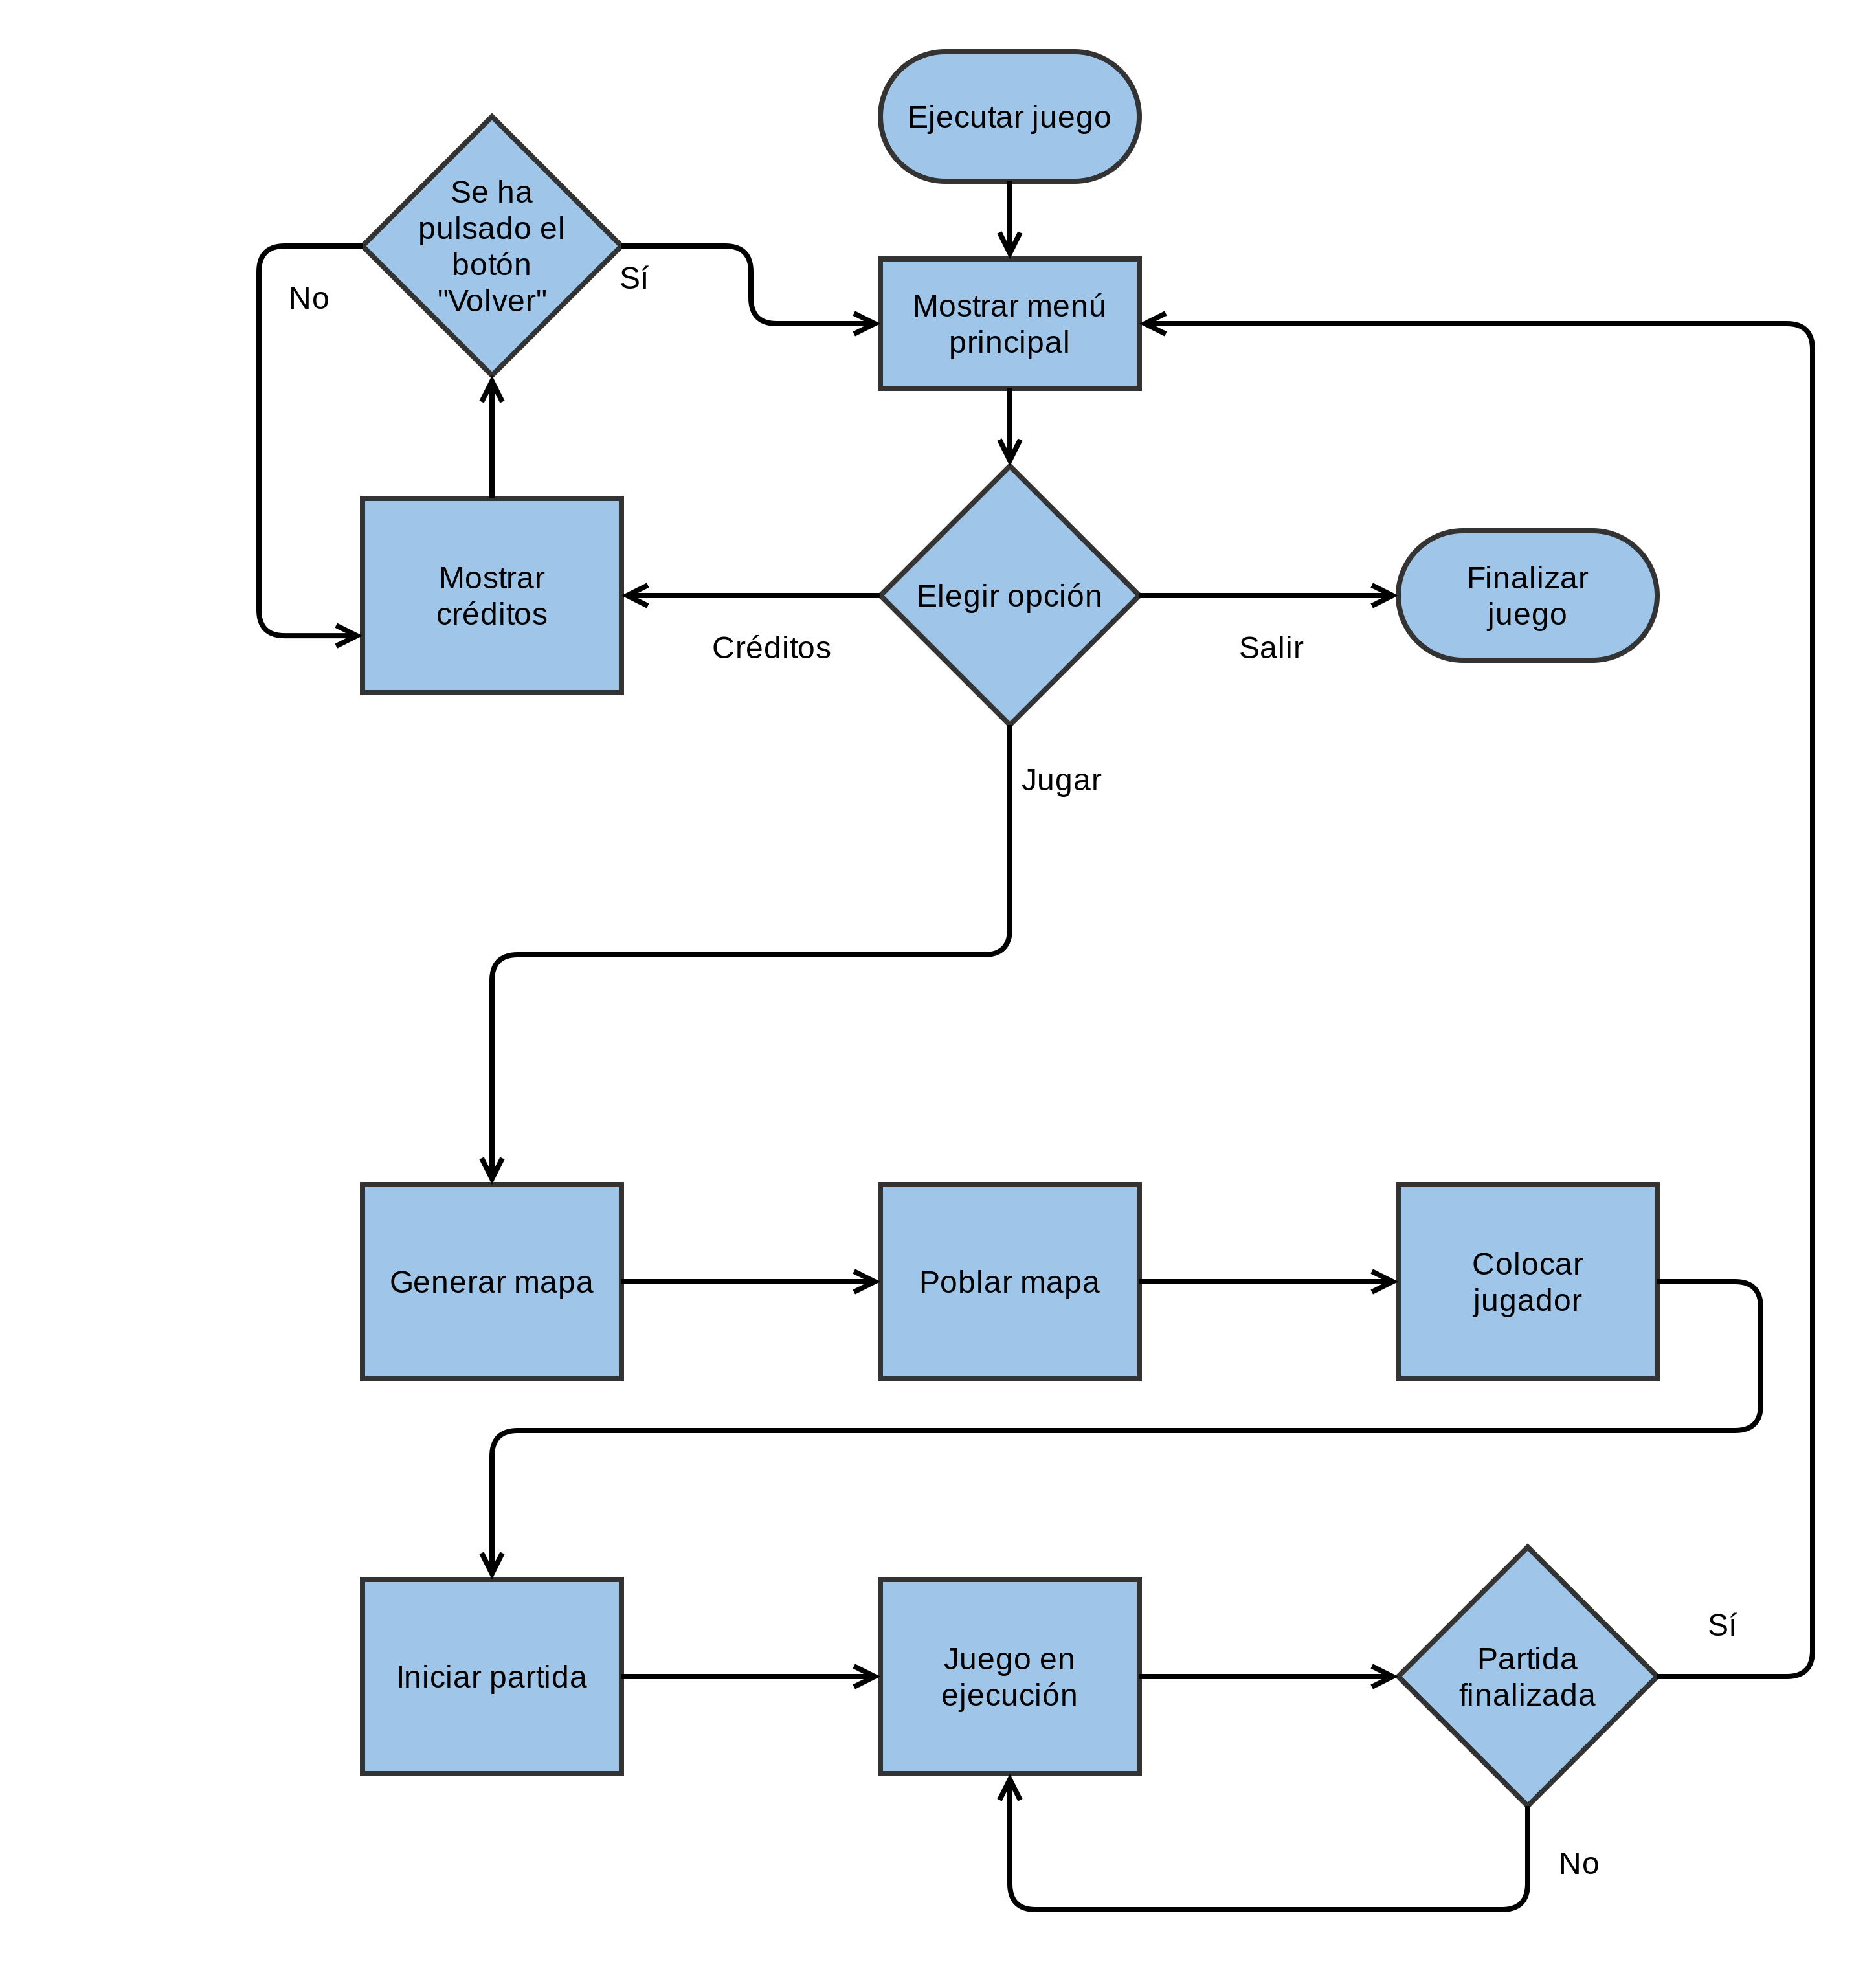
\includegraphics[scale=.13]{fig/actividad}
		 \caption{Diagrama de actividad}
		 \label{fig:activi}
	\end{figure}

	\FloatBarrier

\section{Tecnologías utilizadas}

	En este capítulo se describirán las tecnologías utilizadas para el desempeño del proyecto. Además, se dará una breve explicación de por qué han sido utilizadas y qué beneficios aportan al proyecto.

	\subsection{\acrshort{sfml}}

		\acrfull{sfml}~\cite{sfml} es una librería multiplataforma de desarrollo de software diseñada para proveer una interfaz simple a varios componentes multimedia en ordenadores. Está escrita en C++ con enlaces disponibles para C, D, Java, Python, Ruby, .NET, Go, Rust, OCaml, Euphoria y Nim. Existen también compilaciones experimentales para dispositivos móviles.

		\acrshort{sfml} gestiona tanto la creación e interacción de ventanas como de contextos \acrshort{opengl}. También provee de un módulo grñafico para gráficos acelerados por hardware en 2D el cual incluye representación de texto utilizando FreeType, un módulo de audio que se sirve de \acrshort{openal} y un módulo de conexión para comunicación básica por \acrshort{tcp} y \acrshort{udp}.

		\acrshort{sfml} es un software gratuito y de código libre provisto bajo los términos de la licencia zlib/png. Está disponible para Windows, Linux, OS X y FreeBSD.

		\begin{figure}[!htp]
			 \centering
			 
\includegraphics[scale=.8]{fig/sfml}
			 \caption{Logotipo de \acrshort{sfml}}
			 \label{fig:sfml}
		\end{figure}

		\FloatBarrier

		Se ha decidido utilizar \acrshort{sfml} en el proyecto ya que uno de los objetivos del mismo es aprender a crear una arquitectura software apropiada para videojuegos, de forma que los motores con editor visual no eran una opción, al abstraer al usuario de ella. A pesar de que la librería de referencia para este tipo de aplicaciones es \acrshort{sdl}, se ha decidido usar \acrshort{sfml} ya que a diferencia de la primera, la cual está escrita en C, \acrshort{sfml} está escrita en C++ y concebida con orientación a objetos. Esto supone una ventaja ya que el proyecto ha sido desarrollado en C++ y el paradigma de programación utilizado ha sido el de la orientación a objetos.

	\subsection{C++}

		C++~\cite{cpp} es un lenguaje de programación de propósito general. Tiene características de programación imperativa, orientada a objetos y genérica, mientras provee facilidades para la manipulación de memoria a bajo nivel.

		Está diseñado pensando en la programación de sistemas, sistemas embebidos, sistemas con recursos limitados y grandes sistemas, con el rendimiento, la eficiencia y la flexibilidad de uso como sus requisitos de diseño. C++ también ha sido útil en otros muchos contextos, siendo fortalezas clave la infraestructura de software y aplicaciones con recursos limitados, incluyendo aplicaciones de escritorio, servidores, aplicaciones de rendimiento crítico y software de entretenimiento. C++ es un lenguaje compilado, con implementaciones del mismo disponibles en muchas plataformas y provistas por varias organizaciones, incluyendo \acrshort{fsf}, \acrshort{llvm}, Microsoft e Intel.

		C++ está estandarizado por \acrshort{iso}, con la última versión estándar ratificada y publicada por \acrshort{sfml} en diciembre de 2014 como \acrshort{iso}/\acrshort{iec} 14882:2014 (informalmente conocida como C++14). Muchos otros lenguajes de programación han sido influenciados por C++, entre los que se encuentran C\#, Java, y versiones posteriores a 1998 de C.

		\begin{figure}[!htp]
			 \centering
			 
\includegraphics[scale=.25]{fig/cpp}
			 \caption{Logotipo de C++}
			 \label{fig:cpp}
		\end{figure}

		\FloatBarrier

		Se ha decidido utilizar C++ para el desarrollo del proyecto ya que es el lenguaje estándar de la industria, y dado que el producto busca competir, es importante que esté hecho con las mejores herramientas. C++ es en este caso dicha herramienta, por su eficiencia y flexibilidad.

	\subsection{\acrshort{json}}

		\acrfull{json}~\cite{json} es un formato estándar abierto que usa texto legible por humanos para transmitir objetos de información consistentes en pares atributo-valor. Es principalmente utilizado para transmitir información entre un servidor y una aplicación web como alternativa a \acrshort{xml}.

		Aunque originalmente fue derivado del lenguaje de programación Javascript, \acrshort{json} es un formato de datos independiente del lenguaje. El código necesario para generar y analizar información en \acrshort{json} está disponible en muchos lenguajes de programación.

		\begin{figure}[!htp]
			 \centering
			 
\includegraphics[scale=.5]{fig/json}
			 \caption{Logotipo de \acrshort{json}}
			 \label{fig:json}
		\end{figure}

		\FloatBarrier

		Se ha decidido utilizar \acrshort{json} frente a \acrshort{xml} porque el equipo disponía de experiencia previa con \acrshort{json} y no con \acrshort{xml}. Ambas tecnologías ofrecen características similares, pero \acrshort{json} es más simple y por tanto más fácil de mantener.

	\subsection{\acrshort{tgui}}

		\acrfull{tgui}~\cite{tgui} es una librería de GUI multiplataforma en C++ para \acrshort{sfml}. Entre sus características más destacables encontramos la facilidad de uso, la portabilidad de código, la posibilidad de modificar interfaces sin necesidad de recompilar, un gestor de texturas externo que evita la recarga de imágenes y está provisto bajo la misma licencia que \acrshort{sfml}, zlib/png.

		\begin{figure}[!htp]
			 \centering
			 
\includegraphics[scale=.75]{fig/tgui}
			 \caption{Logotipo de \acrshort{tgui}}
			 \label{fig:tgui}
		\end{figure}

		\FloatBarrier

		Se ha decidido utilizar \acrshort{tgui} en el proyecto para agilizar el desarrollo de las interfaces de usuario. Hubiese sido posible crear una implementación propia con los elementos necesarios, pero hubiese consumido recursos que eran de gran valor para otros apartados del proyecto.

	\subsection{JsonCpp}

		JsonCpp~\cite{jsoncpp} es una librería C++ que permite manipular documentos \acrshort{json}, incluyendo serialización y deserialización a y desde cadenas de texto. También preserva comentarios existentes en los pasos de serialización y deserialización, haciendo el formato conveniente para archivos generados por usuarios.

		De entre las distintas opciones para trabajar con \acrshort{json} en C++, se ha decantado por esta ya que su integración en el proyecto era muy sencilla, al igual que su uso.

\section{Diseño del juego}

	En esta sección se presentará el diseño del juego, es decir, la definición del comportamiento del mismo dentro de una partida.

	\subsection{Jugador}

		El jugador podrá moverse libremente por el mapa y utilizar cualquiera de sus habilidades en todo momento, siempre que no esté ya usando una o esté siendo desplazado por haber sido alcanzado por un ataque enemigo. No existirá límite en el número de veces que puede usar cualquiera de sus habilidades.

		Si el jugador es dañado, su barra de vida, la cual siempre será visible durante una partida, se reducirá en un cuarto. De esta manera, si el jugador es dañado cuatro veces en la misma partida, morirá y la partida se considerará un fracaso. No existirá manera de regenerar la barra de vida.

		El enemigos dispone de tres habilidades: ataque cuerpo a cuerpo, disparo y poantar bomba. Si un jugador colisiona con un enemigo mientras ejecuta el ataque cuerpo a cuerpo y el lado de la colisión coincide con el lado hacia el que está ejecutando el ataque, el enemigo será dañado y el jugador quedará impune. En cualquier otro caso si el jugador es alcanzado por un enemigo o un proyectil enemigo, será dañado.

	\subsection{Enemigos}

		Habrá dos tipos de enemigo en el juego, ambos con el objetivo de acabar con el jugador. Ambos estarán quietos hasta que el jugador entre en su radio de acción, y se quedarán quietos si el jugador sale del mismo.

		El primer enemigo buscará chocarse contra el jugador, de forma que buscará la ruta más corta hasta el mismo y procederá a recorrerla. En caso de que el jugador se mueva volverá a buscar una ruta hasta él. Si el enemigo colisiona con el jugador, lo dañará y lo empujará hacia atrás. Este enemigo morirá si es alcanzado por cualquiera de las habilidades del jugador.

		El segundo enemigo, en vez de buscar una ruta hasta el jugador, buscará la ruta más corta para alienarse con él y la recorrerá. Una vez alineado, disparará al jugador infinitas veces, con un breve espacio de tiempo entre disparo y disparo. Los disparos de este enemigo no podrán ser bloqueados o eliminados de ninguna manera, solo podrán ser esquivados. Este enemigo morirá si es alcanzado por cualquiera de las habilidades del jugador, y tanto sus disparos como su contacto físico directo dañarán al jugador y lo empujarán.

	\subsection{Colisiones con el mundo}

		Tanto el personaje como los enemigos deben colisionar adecuadamente con el mundo, es decir, solo deben ser capaces de atravesar las celdas que, tanto a nivel lógico como visual, son navegables. En caso de que intenten atravesar una celda que no cumpla alguno de los requisitos, el juego debe parar su movimiento y colocarlo justo al lado de la casilla que pretendía atravesar.

	\subsection{Colisiones con objetos}

		Habrá dos objetos con los que se pueda colisionar: proyectiles y bombas.

		Los proyectiles no colisionarán con el mundo, es decir, serán capaces de atravesar cualquier obstáculo. Los proyectiles lanzados por el jugador solo dañarán a enemigos y viceversa.

		Las bombas no podrán ser colocadas en partes del mapa que no se puedan atravesar. Una vez colocadas, permanecerán inactivas un breve periodo de tiempo, y tras esto explotarán. Mientras la bomba está inactiva, no tendrá ninguna consecuencia colisionar con ella. No obstaculizará el movimiento y no dañará. Sin embargo, a la hora de explotar, la caja de colisión de la bomba aumentará y dañará a cualquier cosa que colisione con ella, ya sea un enemigo o el propio jugador.

	\subsection{Objetivo}

		El objetivo del juego es eliminar a todos los enemigos del mapa dentro del tiempo límite fijado. Este tiempo será visible en todo momento en pantalla, y su valor se actualizará cada segundo. Se considerará una partida existosa si el jugador consigue acabar con todos ellos, y se considerará un fracaso si los enemigos consiguen matarlo o se le agota el tiempo límite.

\section{Plan de pruebas}

	Durante la realización del proyecto han habido muchas pruebas para garantizar la calidad del código e intentar minimizar al máximo los errores. En este capítulo se explican las pruebas hechas.

	En la siguiente lista se muestran los tipos de prueba que se han hecho:

	\begin{itemize}
		\item \textbf{Pruebas unitarias:}
			
		Descripción de las pruebas unitarias llevadas a cabo en el proyecto.

		\item \textbf{Pruebas de integración:}
			
		Descripción de las pruebas de integración llevadas a cabo.

		\item \textbf{Pruebas de hardware:}
			
		Descripción de las pruebas de hardware realizadas.

		\item \textbf{Pruebas de usabilidad:}
			
		Descripción de las pruebas de usabilidad realizadas.
	\end{itemize}

	\subsection{Pruebas unitarias}

		A lo largo del proyecto se han realizado muchas pruebas unitarias. Estas consisten en dividir el código a partes mínimas para garantizar que el funcionamiento del mismo es el esperado. La realización de estas pruebas han sido enfocadas a la búsqueda de errores en los siguientes elementos:

		\begin{itemize}
			\item \textbf{Condiciones booleanas:} verificar el comportamiento del sistema al finalizar y asegurar que las variables evaluadas tienen asignados los valores esperados.

			\item \textbf{Indices de matrices:} verificar que en ningún momento se accede a posiciones fuera del rango de las matrices.

			\item \textbf{Comprobar valores nulos:} comprobar que donde se espera que haya una instancia de una clase verdaderamente la haya, de forma que el valor no sea nulo.

			\item \textbf{Operaciones de conversión:} asegurar que la conversión de un tipo a otro de datos es la apropiada, reforzando el código para que una conversión inadecuada cause un error en la aplicación.

			\item \textbf{Condiciones alternativas:} garantizar que al menos una rama es siempre satisfecha.

			\item \textbf{Iteraciones:} asegurar que las condiciones sean correctas de forma que nunca se generen bucle infinitos.

			\item \textbf{Impresión de secuencia:} utilizada para comprobar si la aplicación ejecuta bucles o condicionales imprimiendo la secuencia en consola.
		\end{itemize}

	\subsection{Pruebas de integración}

		La realización de estas pruebas consiste en garantizar que el funcionamiento de cada módulo sea correcto. Los módulos han sido probados de distintas maneras para asegurar que siempre se ejecutaban satisfactoriamente. Además, se han hecho pruebas que verifican que las interfaces de comunicación entre distintos módulos son correctas. Se ha prestado especial atención a este apartado para evitar que el error de un módulo pudiera propagarse a toda la aplicación, evitando así fallos en cadena.

	\subsection{Pruebas de hardware}

		Cuando el producto se encontraba en sus etapas finales, se ha procedido a compilar y ejecutar el juego en distintas configuraciones de hardware para comprobar que funcionaba correctamente. Gracias a la colaboración de compañeros y amigos ha habido posibilidad de probar el producto en una gama variada de hardware. En total se ha compilado y ejecutado el juego satisfactoriamente en catorce configuraciones distintas. Además, estas configuraciones disponían de distintos sistemas operativos, entre los que se encuentran Ubuntu, Linux Mint, Windows 7, Windows 8.1 y OS X. Esto demuestra que el código generado por el proyecto es multiplataforma.

	\subsection{Pruebas de usabilidad}

		Una parte fundamental de los juegos es la experiencia de usuario. Para conseguir la mejor posible, se ha contado con la colaboración de distintas personas que han ayudado a calibrar distintos menúes e interfaces gráficas. Las pruebas consistían en sesiones cortas de juego, en las que los usuarios compartía sus observaciones respecto a la interfaz y usabilidad general. Gracias a las opiniones recogidas, se han ajustado las posiciones y los tamaños de los elementos de la interfaz gráfica para acomodarlos a la mayoría de los usuarios. Por otro lado, se han ajustado los menús para ser más intuitivos.

\chapter{Consideraciones sobre la implementación}

\section{Visión general}

\section{Reglas de estilo}

\section{Entorno de desarrollo}

	Para el desarrollo del proyecto se han utilizado varias herramientas para facilitar la codificación, compilación y búsqueda de errores.

	\subsection{Atom}

		Atom es un editor de texto desarrollado por Github. Es una herramienta que permite personalizar cualquier cosa, pero también permite ser usada productivamente sin tocar ningún archivo de configuración. Atom ofrece integración con Node.js y está diseñado de forma completamente modular, de forma que es posible acoplar un número indefinido de módulos a su núcleo mínimo. Además, su versión más mínima ya dispone de todas las características necesarias para empezar a trabajar. Por último, Atom es de código libre y, por tanto, gratuito.

		\begin{figure}[!htp]
			 \centering
			 
\includegraphics{fig/atom}
			 \caption{Logo de Atom}
			 \label{fig:atom}
		\end{figure}

		Este software ha sido la herramienta principal para el proyecto. Ha sido utilizada para la codificación de todo el proyecto, para el retoque de los archivos JSON y para la generación de los archivos de configuración necesarios. Cualquier editor de texto sencillo podría haber sido utilizado, pero se ha optado por Atom ya que provee características avanzadas para codificar, tales como soporte para distintos lenguajes, que además pueden ser ampliadas mediante módulos gratuitos.

	\subsection{G++}

	\subsection{Git}

		Git es un software de control de versiones diseñado por Linus Torvalds pensando en la eficiencia y la confiabilidad del mantenimiento de versiones de aplicaciones cuando

	\subsection{Make}

	\subsection{Darkfunct Editor}

	\subsection{XML to JSON}

\section{Código y jerarquía de proyecto}

\section{Desarrollo del juego}
\chapter{Plan de Pruebas}

	Durante la realización del proyecto han habido muchas pruebas para garantizar la calidad del código e intentar minimizar al máximo los errores. En este capítulo se explican las pruebas hechas.

	En la siguiente lista se muestran los tipos de prueba que se han hecho:

	\begin{itemize}
		\item \textbf{Pruebas unitarias:}
			
		Descripción de las pruebas unitarias llevadas a cabo en el proyecto.

		\item \textbf{Pruebas de integración:}
			
		Descripción de las pruebas de integración llevadas a cabo.

		\item \textbf{Pruebas de hardware:}
			
		Descripción de las pruebas de hardware realizadas.

		\item \textbf{Pruebas de usabilidad:}
			
		Descripción de las pruebas de usabilidad realizadas.
	\end{itemize}

\section{Pruebas unitarias}

	A lo largo del proyecto se han realizado muchas pruebas unitarias. Estas consisten en dividir el código a partes mínimas para garantizar que el funcionamiento del mismo es el esperado. La realización de estas pruebas han sido enfocadas a la búsqueda de errores en los siguientes elementos:

	\begin{itemize}
		\item \textbf{Condiciones booleanas:} verificar el comportamiento del sistema al finalizar y asegurar que las variables evaluadas tienen asignados los valores esperados.

		\item \textbf{Indices de matrices:} verificar que en ningún momento se accede a posiciones fuera del rango de las matrices.

		\item \textbf{Comprobar valores nulos:} comprobar que donde se espera que haya una instancia de una clase verdaderamente la haya, de forma que el valor no sea nulo.

		\item \textbf{Operaciones de conversión:} asegurar que la conversión de un tipo a otro de datos es la apropiada, reforzando el código para que una conversión inadecuada cause un error en la aplicación.

		\item \textbf{Condiciones alternativas:} garantizar que al menos una rama es siempre satisfecha.

		\item \textbf{Iteraciones:} asegurar que las condiciones sean correctas de forma que nunca se generen bucle infinitos.

		\item \textbf{Impresión de secuencia:} utilizada para comprobar si la aplicación ejecuta bucles o condicionales imprimiendo la secuencia en consola.
	\end{itemize}

\section{Pruebas de integración}

	La realización de estas pruebas consiste en garantizar que el funcionamiento de cada módulo sea correcto. Los módulos han sido probados de distintas maneras para asegurar que siempre se ejecutaban satisfactoriamente. Además, se han hecho pruebas que verifican que las interfaces de comunicación entre distintos módulos son correctas. Se ha prestado especial atención a este apartado para evitar que el error de un módulo pudiera propagarse a toda la aplicación, evitando así fallos en cadena.

\section{Pruebas de hardware}

	Cuando el producto se encontraba en sus etapas finales, se ha procedido a compilar y ejecutar el juego en distintas configuraciones de hardware para comprobar que funcionaba correctamente. Gracias a la colaboración de compañeros y amigos ha habido posibilidad de probar el producto en una gama variada de hardware. En total se ha compilado y ejecutado el juego satisfactoriamente en catorce configuraciones distintas. Además, estas configuraciones disponían de distintos sistemas operativos, entre los que se encuentran Ubuntu, Linux Mint, Windows 7, Windows 8.1 y OS X. Esto demuestra que el código generado por el proyecto es multiplataforma.

\section{Pruebas de usabilidad}

	Una parte fundamental de los juegos es la experiencia de usuario. Para conseguir la mejor posible, se ha contado con la colaboración de distintas personas que han ayudado a calibrar distintos menúes e interfaces gráficas. Las pruebas consistían en sesiones cortas de juego, en las que los usuarios compartía sus observaciones respecto a la interfaz y usabilidad general. Gracias a las opiniones recogidas, se han ajustado las posiciones y los tamaños de los elementos de la interfaz gráfica para acomodarlos a la mayoría de los usuarios. Por otro lado, se han ajustado los menús para ser más intuitivos.

\chapter{Incidencias}
\chapter{Conclusiones y Líneas Futuras}

\section{Visión general}

	Este capítulo recoge, a modo de conclusión, la visión del equipo de trabajo tras la realización del proyecto, expresando sus opiniones acerca del trabajo realizado teniendo en cuenta contribuciones personales y desarrollo profesional.

\section{Objetivos cumplidos}

	A pesar de no contar con tanto tiempo como se hubiese deseado para la realización del proyecto debido a diversas responsabilidades, se podría considerar que los objetivos del proyecto han sido cumplidos, tal como se definen en el capítulo correspondiente.

	\begin{itemize}

		\item Se ha desarrollado un producto jugable y estable.

		\item Las características principales están implementadas.

		\item La arquitectura del software está preparada para añadir y modificar con facilidad nuevas funciones.

		\item La investigación hecha para desarrollar del proyecto ha permitido aprender mucho sobre el desarrollo de soluciones software de este tipo.

		\item Se han aprendido técnicas y patrones de diseño utilizados comúnmente en la industria, y se han implementado algunos de ellos.

		\item El producto está en una fase que, si se añadiesen más funcionalidades y otras características de juegos, podría comercializarse.

	\end{itemize}

	Por otro lado, los requisitos definidos del software han sido cumplidos también:

	\begin{itemize}
			\item
				
			El nivel es generado proceduralmente en cada sesión y es poblado de enemigos.
			
			\item 
				
			El juego es capaz de detectar cuando distintas entidades colisionan entre ellas o con el escenario y actúa en consecuencia.

			\item 
				
			La cámara del juego sigue al jugador en los ejes X e Y.

			\item 
				
			El juego detecta las entradas del jugador, comprueba el estado actual del mismo y actúa en consecuencia.

			\item 
				
			El juego detecta cuando se han cumplido las condiciones para fin de partida y la termina.

			\item 
				
			Cada enemigo tiene una inteligencia artificial distinta.

			\item 
				
			El jugador tiene a su disposición tres tipos de ataque.

			\item 
				
			El juego cuenta con una pantalla para mostrar los controles.

			\item
					
			Durante las partidas el juego muestra en todo momento los datos relevantes al usuario mediante una interfaz gráfica.

			\item
				
			La interfaz gráfica no molesta al jugador.

			\item
				
			El juego se controla únicamente con el teclado.

			\item 
				
			El código del juego es multiplataforma, de forma que puede compilarse en Windows, Linux y OSX.

			\item 
				
			La versión final incluye las librerías necesarias para el correcto funcionamiento del juego.

			\item
					
			El juego funciona a un mínimo de 30 \acrshort{fps} en cualquier plataforma.

			\item
				
			Durante las partidas, no hay errores que provoquen un final inesperado de la aplicación.
	\end{itemize}

\section{Consideraciones del trabajo realizado}

	Este proyecto nació de la afición a los videojuegos y del deseo a crearlos. Desde siempre el alumno ha sido un gran aficionado a jugar a estos producto, y a medida que jugaba se iba interesando más y más por ellos. Ya desde pequeño, tras pasar las épocas de astronauta y bombero, el alumno decía que se quería dedicar a ello, y con el paso de los años esa decisión no hizo más que reafirmarse. Existen muchas maneras de entrar a formar parte del mundo del desarrollo de videojuegos, pero todos los profesionales coinciden en que, a pesar de que existen ofertas formativas muy buenas, sin duda la mejor manera es simplemente haciendo juegos. Con esto en mente, el alumno se lanzó a desarrollar el proyecto con la esperanza de que fuese la mejor experiencia educativa posible.

	Para desarrollar el proyecto, el alumno tuvo que considerar una serie de aspectos. El primero fue el lenguaje de programación, ya que sería la herramienta principal del desarrollo, y la elección del mismo tendría gran repercusión. Dado que C++ es el lenguaje utilizado profesionalmente para el desarrollo de juegos, el alumno se decantó por el mismo, ya que aspira a ser un profesional del área. Además, en el grado obtuvo unas nociones básicas del mismo, de forma que la curva de aprendizaje se vería aligerada. Tras esto, comparó distintos motores y frameworks, y finalmente se decantó por \acrshort{sfml} ya que está escrito en C++ y permitía al alumno desarrollar el software a su antojo. El alumno no tenía ninguna experiencia previa con \acrshort{sfml}, de forma que tuvo que pasar por una fase de aprendizaje.

	Para asimilar el aprendizaje teórico, el alumno desarrolló unos cuantos programas pequeños para hacer con \acrshort{sfml}, de esta forma se familiarizó con la librería y fue capaz de detectar errores e inconveniencias. Para solucionarlos y mejorar su uso de la librería, se sirvió de la comunidad de \acrshort{sfml}, accediendo a su foro, su wiki y a otros recursos encontrados en internet.

	Por otro lado, el alumno no tenía conocimiento alguno sobre la generación procedural. Sin embargo, era un área en la que estaba muy interesado, porque el hecho de ofrecer una experiencia única en cada partida lo seducía. Por ello, se lanzó a investigar sobre distintos algoritmos de generación, enfocándose principalmente en los de generación de mapas. En este punto huelga decir que el alumno se sorprendió con la cantidad de recursos que había al respecto, no se esperaba encontrar tantísima información. Tras barajar distintas posibilidades, se decantó por utilizar un algoritmo que, pese a su sencillez, otorga unos resultados muy satisfactorios. Esta decisión se tomó en base a que por desgracia no se disponía tanto tiempo como se hubiese deseado para el desarrollo.

	En general, hay que decir que pese a que se poseía conocimiento previo respecto a muchas áreas utilizadas como la programación, manipulación gráfica o el desarrollo de videojuegos, el alumno considera que ha sido una experiencia muy enriquecedora, y que gracias a ella ha aprendido un montón de técnicas y ha descubierto muchos recursos de aprendizaje nuevos que, aunque no ha podido utilizarlos todos en el desarrollo de este proyecto, sin duda serán de gran ayuda y de un valor incalculable para el futuro.

\section{Líneas Futuras}

	Aunque se han completado todos los objetivos definidos para el proyecto, hay ciertas extensiones que se podrían llevar a cabo para mejorar el producto. El juego se puede extender con múltiples características, algunas de ellas podrían ser:

	\begin{itemize}

		\item Habilidades: Sería interesante que el jugador tuviese a su disposición más herramientas con las que interactuar con el juego. Además, podría crearse un sistema que le permitiese mejorar las habilidades que ya tuviese y asignarlas a los controles que prefiera. Por suerte este tipo de cambios estaban previstos para el futuro, y la arquitectura del software está pensada para que sea sencillo y seguro añadir más elementos de este tipo.

		\item Generación de mapas: En la versión actual siempre se utiliza el mismo algoritmo para generar mapas. A pesar de que los resultados son bastante variados, añadir distintos algoritmos de generación supondrían un valor añadido al proyecto. Nuevamente, el software está preparado para soportar cambios de estas características.

		\item Enemigos: Al solo existir dos tipos de enemigos, el juego es bastante monótono. Por ello, añadir más enemigos con comportamientos únicos añadiría dinamicidad y diversión al juego. Por otro lado, se podría pensar en crear enemigos más poderosos, con una \acrshort{ia} única, que podrían ser enemigos finales para los niveles. Una vez más, el software está pensado para añadir nuevos enemigos con facilidad, aunque habría que diseñar la parte relativa a los nuevos enemigos únicos.

		\item Historia: A pesar de que en el pasado prácticamente todos los juegos fuesen arcade y no tuviesen apenas historia, hoy en día la narrativa de un juego tiene la misma o más importancia que la jugabilidad. Por ello, desarrollar una historia para el juego e implementar elementos para poder contarla adecuadamente sería muy enriquecedor. Los elementos a añadir serían cuadros de diálogo para los personajes, un sistema de secuencias etc.

	\end{itemize}

	Si todas o algunas de las extensiones fuesen llevadas a cabo, sin duda el producto final sería de una calidad notable, lo cual se traduce en que podría ser puesta en venta al público y haría competencia con otros juegos del mismo corte.
	

\printbibliography[heading=bibintoc]
\printglossary[type=\acronymtype, title=Acrónimos, toctitle= Acrónimos]

\appendix

\chapter{Manual de usuario}

	\section{Menú principal}

		Al ejecutar la aplicación, se le muestra al usuario un menú principal. Dicho menú cuenta con tres opciones:

		\begin{itemize}

			\item Jugar

				Esta opción dará comienzo a una partida. El jugador será traslado a la pantalla de juego, donde se desarrollará la partida.

			\item Créditos

				Esta opción mostrará la pantalla de créditos, la cual contará con un botón \textit{Atrás}, el cual devolverá al usuario al menú principal.

			\item Salir

				Esta opción cerrará la aplicación.

		\end{itemize}

	\section{Objetivo}

		Una vez dentro de la partida, existen dos formas de finalizarla:

		\begin{itemize}		

			\item \textbf{Eliminando a todos los enemigos}: El jugador, valiéndose de las tres habilidades de las que dispone, debe acabar con todos los enemigos que hay en el nivel. Si lo consigue, la partida terminará y el jugador será enviado de vuelta al menú principal automáticamente.

			\item \textbf{Excediendo el tiempo de partida}: Alternativamente, si el jugador pasa demasiado tiempo sin conseguir eliminar a todos los enemigos del nivel y la cuenta atrás mostrada en pantalla llega a cero, la partida finalizará automáticamente, devolviendo al jugador al menú principal.

		\end{itemize}

	\section{Controles}

		El jugador, para interactuar con el juego, debe utilizar el siguiente esquema de controles:

		\begin{itemize}

			\item En el menú principal, el usuario debe interactuar con los botones mediante el ratón, es decir, para seleccionar cualquier de las opciones, debe hacer click en el botón correspondiente.

			\item Una vez en partida, el resto de las entradas se realizan mediante el teclado. Para moverse por el escenario, el jugador debe utilizar las teclas direccionales. Para utilizar sus habilidades, deberá utilizar las teclas \textit{A}, \textit{S} o \textit{D} en función de la que quiera ejecutar.

			\begin{itemize}

				\item \textbf{A}: Disparar flecha.

				\item \textbf{S}: Colocar bomba.

				\item \textbf{D}: Ataque cuerpo a cuerpo.

			\end{itemize}

		\end{itemize}
\chapter*{Agradecimientos}
\addcontentsline{toc}{chapter}{Agradecimientos}

No quisiera finalizar esta memoria sin dar las gracias a todas aquellas personas que me han apoyado durante estos meses de trabajo. En especial quisiera dar las gracias a:

\begin{itemize}

	\item \textbf{Mis padres}, por darme la vida, mantenerme (a pesar de haber salido tonto) y haberme dado la oportunidad de hacer lo que quería y apoyarme en todo momento (menos cuando me quise dejar el pelo largo, ahí tuve que pelear).

	\item \textbf{Andoni Eguíluz Morán}, por aceptar dirigir el proyecto y por la ayuda y buen trato que siempre he recibido de su parte.

	\item \textbf{Mis compañeros y amigos}, tanto de la facultad como de fuera de ella. Por animarme en los momentos de bajón, aguantar mis chapas e idas de olla y ayudarme cuando lo he necesitado. Y todo ello sin pagarles nada.

	\item \textbf{Desarrolladores de videojuegos}, especialmente indies, por la gran inspiración que han supuesto y sin la cual seguramente este proyecto ni siquiera hubiese nacido.

	\item \textbf{Mi estructura ósea}, por el apoyo que me ha proporcionado todos estos años.

\end{itemize}

Y en general a toda persona, ya sea amigos, compañeros, desarrolladores, artistas, músicos, directores de cine, actores, actrices, médicos, carpinteros, fontaneros, camareros, barrenderos, dependientes de tiendas de animales, profesores, estudiantes, ninis, técnicos de televisión, ingenieros de lavavajillas, pregoneros, abogados, arquitectos, carniceros, cirujanos, dentistas, fotógrafos, jardineros, modelos, psiquiatras, soldados, taxistas, caballeros andantes, recepcionistas, veterinarios, panaderos, enfermeros, electricistas o bomberos que, ya sea directa o indirectamente, hayan conseguido sacarme una sonrisa durante este último año. De verdad, a todos, gracias de corazón.

\backmatter

\end{document}
